In this chapter, we propose a new sample-efficient training method, called \emph{amplified negative sampling}, for training multi-class classifiers with a large output-class size. Our method jumps out of the framework of softmax appximation and directly tackle the optimum convergence point of the learning algorithm. Our proposed method is based on our  analysis of the well-known negative sampling technique~\citep{mikolov2013distributed} and is designed for (1) higher performance in the general task and (2) lower training computational cost. Our experiments on real-world datasets demonstrate that our proposed method leads to sampling cost savings with performance boost compared to the standard technique.

\section{Introduction}

In this work,we provide a novel sample-efficient method for training a multi-class classifier $C: X \rightarrow Y$ ($X$: input features, $Y$: output class labels) when the output-class size is large, say, $\vert Y \vert = 50,000$. Typically, when a classifier is modeled as a neural network, the final layer is implemented as a softmax layer with \emph{one output neuron per each output class label} $y \in Y$, making it prohibitively expensive to train even for a reasonably large output-class size. To address this computational challenge, a number of techniques have been proposed, such as hierarchical softmax~\citep{morin2005hierarchical},negative sampling~\citep{mikolov2013efficient}, adaptive softmax~\citep{bengio2008adaptive} and its variants~\citep{rawat2019sampled,blanc2017adaptive,grave2017efficient,chen2015strategies,bai2017tapas}. Due to its simplicity and efficiency, negative sampling is one of the most popular techniques used in practice~\citep{mikolov2013distributed,wang2017knowledge,node2vec-kdd2016,barkan2016item2vec}. In particular, it is widely utilized in many embedding frameworks, such as word embedding~\citep{mikolov2013distributed}, graph embedding~\citep{node2vec-kdd2016,wang2017knowledge}, and product-user embedding~\citep{barkan2016item2vec}.


The key idea behind negative sampling is as follows: Given a training data point $(x_i, y_i)$, the standard training algorithm updates the weights of the output neurons for \emph{all} $y\text{'s} \in Y$, not just for the training label $y_i$, making the training cost proportional to the output-class size $\vert Y \vert$. Negative sampling avoids this high cost by adjusting the weights for (1) the given training label, $y = y_i$ (``the positive sample'') and (2) just a few $y\text{'s}$ that are randomly sampled from $Y - \{y_i\}$ (``negative samples''). Clearly, taking a few negative samples reduces the training cost by several orders of magnitudes when the output class size is large. 

In general, it is reported that using a larger negative sample size leads to better downstream performance. For example, when Mikolov used negative sampling to embed words into high-dimensional vectors in~\citep{mikolov2013distributed}, he reported between 2-15\% increase in downstream task performance when he used the 15 negative samples ($k=15$) compared to 5 negative samples ($k=5$). Unfortunately, the training cost of $k=15$ is three times as large as that of $k=5$, making its use significantly less appealing in practice. For instance, since training on a larger corpus generally improves the downstream performance as well, it may be the case that using a smaller $k$ on a larger corpus may be just as good as or even better than using a larger $k$ on a smaller corpus. This is the primary topic of this chapter. Is it possible to get the best of both worlds? Can we achieve a higher-quality model trained on a larger $k$ without paying its training cost?

%To obtain an answer to this question, we first conduct a rigorous mathematical analysis of the impact of the negative-sampling technique on the accuracy of the learned model. The result of this analysis will show exactly how negative sampling affects the accuracy of the learned model and provide theoretical explanations for a few empirical observations that have been well known among practitioners. It will also shed light on how it can be further improved for higher training efficiency. Based on this insight, 

In this chapter, we give our answer to this question by finding a surprisingly simple yet effective  modification to the negative sampling technique, named \emph{amplified negative sampling}.  Compared to the standard negative-sampling technique, our proposed technique can be used to either (1) \emph{improve the prediction accuracy} of the trained model \emph{for the same training cost} or (2) \emph{lower the training cost for the same prediction accuracy}. We demonstrate the effectiveness of our proposed technique through extensive experiments on real-world data sets.

In summary, we make the following contributions in this chapter:
%	\item We provide a rigorous mathematical analysis of the impact of negative sampling on the trained model under the three most popular loss functions, $L1$, $L2$, and cross entropy. As far as we know, our work is the first that derives the exact analytical form of the global optimal points when the classifier is trained with negative sampling under the three popular loss functions. The result of our analysis provides a clear understanding of the implication of negative sampling. 
	%For example, we prove that the optimal model trained with the $L2$ loss function is the same as that with the \emph{cross entropy} loss function. We also show that the optimal model trained with the $L1$ loss function is a sparse binary model. 
(\romannum{1}) We propose \emph{amplified negative sampling}, a simple yet effective modification to the widely-used negative-sampling technique that can improve its accuracy and lower its training cost based on our rigorous mathematical analysis.
 (\romannum{2}) We compare the effectiveness of our proposed technique with standard negative sampling by conducting an extensive set of experiments on real-world data sets. Our results show that the effectiveness of our technique is in line with our theoretical prediction and can often be \emph{twice as sample efficient} as the standard technique. 


The rest of this chapter is organized as follows. In Section~\ref{sec:NS:framework}, 
we formally describe the multi-class classification problem and review the standard negative sampling technique. Then in Section ~\ref{sec:NS:amplified}, 
we propose amplified negative sampling and give the rigourous matematical analysis of the method. In Section ~\ref{sec:NS:exp}, 
we present the results of our experiments. We review related work in Section~\ref{sec:NS:related} 
and wrap up the chapter in Section~\ref{sec:NS:conclusion}.

\section{Related Work}
\label{sec:NS:related}
Softmax has been widely used in various models. In large output class classification problem, the intractable normalizing constant of softmax function will slow down the computation efficiency greatly. There are three major types of strategies have been investigated by the research community, including sampled softmax\citep{bengio2008adaptive}, hierarchical softmax\citep{morin2005hierarchical} and spherical softmax\citep{vincent2015efficient}.
We are not aiming to approximate the softmax function. This work makes one related yet distinct contribution: an efficient training method based on negative sampling strategy for a large classifier.  The \citep{ruiz2018augment} share a similar scope with us which is not targeting on softmax appximation. Since the amplifying factor is distribution agnostic, this method actually can be applied to all the sampling-based softmax approximation method\citep{blanc2017adaptive,rawat2019sampled}.

\textbf{Sampled Softmax} This category contains the method which generates a subset of negative samples to avoid the high overhead of full negative sampling. Among this category, one class of methods try to generate samples from the softmax distribution. An adaptive sampling method was proposed by Bengio~\citep{bengio2008adaptive} inspired by the importance sampling. Another prominent example is the negative sampling~\citep{mikolov2013efficient} which uses a simple noisy distribution to generate negative samples. TAPAS~\citep{bai2017tapas} uses a two pass scheme to generate samples from two different size candidate pools to reduce the sample overhead. Hashing method~\citep{bakhtiary2015speeding, vijayanarasimhan2014deep} is also applied to either find the closest class or partial computation.  ~\citep{rawat2019sampled}. 
Another class of methods instead focus on the sampled loss, including Noisy Contrastive Estimation(NCE)~\citep{NCE} by assuming the partition as an extra parameter to be computed during the computation and Adversarial Contrastive Estimation(ACE)~\citep{bose2018adversarial} and ~\citep{schroff2015facenet,mussmann2017fast} selects the hardest negative examples.

\textbf{Hierachical Softmax}
Hierarchical softmax was introduced in ~\citep{Goodman} by utilizing the cluster structure to reduce the computation cost of softmax function. Bengio~\citep{morin2005hierarchical} extend it into the tree structure. Due to the different inference procedure, the hierarchical softmax need extra steps to update the tree structure and maintain its property. Various method are proposed to stabilize this process such as class similarity, frequency binning and other optimization techniques. Zweig did some experiments to compare various  tree structures. 

\textbf{Spherical softmax and kernel method}
The spherical softmax was proposed in ~\citep{vincent2015efficient,de2015exploration} which use quadratic function to replace the exponential function and enable faster computation of the gradients. However, these method seems not quite stable when the output label size is large. Kernel-based methods are also explored in ~\citep{blanc2017adaptive,rawat2019sampled}. These works introduces quadratic kernel and random Fourier features which show very promising results.
\section{Framework}
\label{sec:NS:framework}
In this section, we briefly go over the general problem formulation of multi-class classifier learning and negative sampling to introduce key notation used in this chapter.
\subsection{Preliminaries}
We are given a dataset $D = \{(x_1, y_1),$$(x_2, y_2),$$..., (x_n, y_n)\}$, where $x_i \in X$ is an \emph{input feature} and $y_i \in Y$ is an \emph{output class label}. We assume a discrete space of feature values $x_i$ and output labels $y_i$, such that $x_i$ and $y_i$ take an integer value between $1 \le x_i \le m$ and $1 \le y_i \le m$. The multi-class classifier learning problem is to find a classifier $C: X \rightarrow Y$ that returns the correct label $y_i$ given the input feature $x_i$: $y_i = C(x_i)$. Due to noise in the dataset and the uncertainty in predicting the correct label, this problem is often formulated as finding a conditional probability distribution $P(y|x)$ from the dataset $D$, which is interpreted as the probability that the correct output label is $y$ given the input feature $x$.

Note that this formulation encompasses not just the multi-class classifier learning problem, but also most of the ``data embedding'' problems, such as word embedding~~\citep{mikolov2013efficient,mikolov2013distributed}, graph embedding~~\citep{grover2016node2vec}, and item embedding~~\citep{barkan2016item2vec}. For example, the well-known skip-gram model for word2vec~~\citep{mikolov2013distributed} falls under this formulation by defining a \emph{context word} as an  input feature $x_i$ and any \emph{target word} that appears near the context word as an output label $y_i$.

Learning the conditional probability function $f(x,y) = P(y|x)$ from the dataset $D$ is done by assuming a parameterized hypothesis space $f_{\theta}(x,y) = P_{\theta}(y|x)$, where the hypothesis space $f_{\theta}: (x, y) \rightarrow [0,1]$ is a space of differentiable functions parameterized by $\theta \in R^d$. Among all possible parameters $\theta \in R^d$, an \emph{optimal parameter $\theta^*$} is chosen to minimize the loss function $L(f_{\theta}, D)$, where $L(f_{\theta}, D)$ captures the ``loss of $f_{\theta}$'' or the difference between $f_{\theta}$ and $D$. Multiple definitions of the loss function $L(f_{\theta},D)$ are used in practice, including $L1$, $L2$, and \emph{cross entropy}:
\vspace{-0.7ex}
\begin{align}L_1:& \sum_{(x_i,y_i)\in D} \sum_{y \in Y} \vert\mathbbm{1}(y=y_i) - f_{\theta}(x_i, y)\vert\\
L_2:& \sum_{(x_i,y_i)\in D} \sum_{y \in Y} (\mathbbm{1}(y=y_i) - f_{\theta}(x_i, y))^2\\
%\end{align}\vspace{-1ex}\begin{align}
L_{\textit{CE}}:&
-\!\!\!\!\!\!\sum_{(x_i,y_i)\in D} \sum_{y \in Y} \left[\mathbbm{1}(y=y_i) \log f_{\theta}(x_i, y) \right. \nonumber\\
&\left. \qquad\,\,\,\,\,\,\,+\left(1 - \mathbbm{1}(y=y_i)\right) \log\left(1 - f_{\theta}(x_i, y)\right)\right] 
\end{align}
%\begin{equation}
%\begin{split}
%   L_1: \sum_{(x_i,y_i)\in D} \sum_{y \in Y} \vert\mathbbm{1}_{y=y_i}(y) - f_{\theta}(x_i, y)\vert
%   L_2: \sum_{(x_i,y_i)\in D} \sum_{y \in Y} (\mathbbm{1}_{y=y_i}(y) - f_{\theta}(x_i, y))^2 
%   L_{\textit{cross-entropy}}: 
%    - \sum_{(x_i,y_i)\in D} \sum_{y \in Y} \left[\mathbbm{1}_{y=y_i}(y) \log f_{\theta}(x_i, y) 
%    \left(1 - \mathbbm{1}_{y=y_i}(y)\right) \log\left(1 - f_{\theta}(x_i, y)\right)\right]
%\end{split}

%\end{equation}
Here, $\mathbbm{1}(y=y_i)$ is an indicator function that takes the value $1$ if $y = y_i$ and $0$ otherwise. In order to make our discussion concrete, we primarily assume $L2$ as our loss function in the rest of this chapter and simply state the result of our analysis for the other loss functions. 

The gradient-descent method is often utilized to identify the parameter $\theta^*$ that minimizes the loss function $L(f_{\theta}, D)$. Given the definition of the $L2$ loss function, its gradient is:
\small
\begin{align}
&\nabla_{\theta} L_2(f_{\theta},D) = 
 -2\!\!\!\!\!\!\sum_{(x_i,y_i)\in D} \!\!\left[\sum_{y \in Y} 
(\mathbbm{1}(y=y_i) - f_{\theta}(x_i, y)) \nabla_{\theta} f_{\theta}(x_i, y)\right] \label{eq:allneg}    
\end{align}
\normalsize
Note that the inner summation of the above equation makes its computation prohibitively expensive: For each training data $(x_i, y_i) \in D$, we take the inner sum over \emph{every} output label $y \in Y$, not just the training label $y_i$.\footnote{In certain cases, this sum over every $y \in Y$ is implicitly added to the hypothesis space $f_{\theta}(x,y)$. For example, when implemented as a neural network, the final layer is typically implemented as a softmax layer with one neuron per output label, which has the same effect as summing over ever $y \in Y$.} This makes the computational cost \emph{proportional to the output class size $|Y|$}. We refer to the training method that computes the full gradient of Equation~\ref{eq:allneg} as \emph{full-gradient training}. 

\subsection{Negative Sampling}
\label{sec:negative}
\emph{Negative sampling} is a technique that tries to reduce the high computational cost of full-gradient training. The idea of negative sampling was originally proposed in 2010 as Noisy Contrastive Estimation (NCE)~~\citep{NCE}, which was generalized for natural language processing by Mihn in~~\citep{mnih2012fast}. It was used as part of the word2vec computation~~\citep{mikolov2013efficient}, which led to a wide adoption for general vector-embedding problems~~\citep{node2vec-kdd2016,barkan2016item2vec,grover2016node2vec}.

The basic idea of negative sampling can be summarized as follows: Given a training data $(x_i, y_i)$, we refer to $y_i$ as the ``\emph{positive sample}'' and all other label $y \in Y - \{y_i\}$ as ``\emph{negative samples}.''  Full-gradient training sums up the gradients from (1) the positive sample $y_i$ and (2) \emph{all} negative samples $y (\neq y_i)$. Negative sampling, instead, sums up the gradients from (1) the positive sample $y_i$ and (2) \emph{just a few randomly-selected negative samples $y \in Y- \{y_i\}$}.

More precisely, we use NEG-$k(i)$ to represent the $k$ randomly-chosen negative samples for the $i$th training data $(x_i, y_i)$. 
That is, NEG-$k(i)$ is a size-$k$ random subset of $Y - \{y_i\}$. Negative sampling then \emph{approximates} the $L2$ loss function $L_2(f_{\theta},D)$ as follows:
\begin{align} 
& L_2(f_{\theta},D) \nonumber\\ 
& =\sum_{(x_i,y_i)\in D} \left[  \sum_{y \in Y} (\mathbbm{1}(y=y_i) - f_{\theta}(x_i, y))^2\right] \label{eq:l2-neg-1}\\
& =\sum_{(x_i,y_i)\in D} \left[ (\mathbbm{1}(y=y_i) - f_{\theta}(x_i, y))^2 \Bigg|_{y=y_i} \right. \nonumber\\
&                           \left. \qquad\qquad\;\;\;\;\;\;\; +\sum_{y \in Y - \{y_i\}} (\mathbbm{1}(y=y_i) - f_{\theta}(x_i, y))^2\right] \label{eq:l2-neg-2}\\
& \approx \!\!\!\!\!\sum_{(x_i,y_i)\in D}\!\left[ (1 - f_{\theta}(x_i, y_i))^2  + \sum_{y \in \text{NEG-$k$}(i)} f_{\theta}(x_i, y)^2 \right] \label{eq:neg-k}
\end{align}
From Equation~\ref{eq:l2-neg-1} to~\ref{eq:l2-neg-2}, the sum over $y \in Y$ is expanded into the sum of $y = y_i$ and $y \in Y - \{y_i\}$. From Equation~\ref{eq:l2-neg-2} to~\ref{eq:neg-k}, the sum over all negative samples $y \in Y - \{y_i\}$ is approximated by the sum over NEG-$k(i)$.
Clearly, this approximation can decrease the cost of computing the loss function significantly when $|Y|$ is large, which is the key reason for its efficiency. But what is the accuracy of this approximation? Will we still be able to get the same accurate model despite this approximation? If not, what is its exact impact? The next section will show the answers for those issues.
%In the next section, we investigate this issue analytically.

\subsection{Optimal Model of Negative Sampling and Full-gradient  Model}

In this section, we investigate the achievable optimal model of the NEG-$k(i)$ and compare it with the model training with all $Y - \{y_i\}$ negative samples (Full-gradient) to see how accurate the NEG-$k(i)$ can approximate. For a better explanation, we use $\#(x)$ to represent the number of times that the input feature value $x$ appears in the training data $D$ and $\#(x,y)$ to represents the number of times that the feature-and-label-value pair $(x,y)$ appears in $D$. More formally,
\small
\begin{align*}
\#(a)   &= \big\vert \{(x, y) \in D \mid x = a \}\big\vert \\
\#(a,b) &= \big\vert \{(x, y) \in D \mid x = a \text{ and } y = b\}\big\vert
%\#(x)   &= \big\vert \{(x_j, y_j) \in D \mid x_j = x \}\big\vert \\
%\#(x,y) &= \big\vert \{(x_j, y_j) \in D \mid x_j = x \text{ and } y_j = y\}\big\vert
\end{align*}
\normalsize
When we select the $k$ negative samples for the $i$th training data $(x_i, y_i)$, NEG-$k(i)$, we assume that a negative sample $y \in Y - \{y_i\}$ is sampled with replacement with probability $p_{y}$. Two popular choices of the sampling probability $p_{y}$ are (1) the uniform distribution $p_{y} = c$ for some constant $c$ and (2) according to the frequency of $y$ in $D$. Our results are stated with the generic symbol $p_y$ without making any explicit assumption on the sampling distribution. With this notation, we now could show the analysis to the negative sampling.
\begin{theorem}[Optimal Model of Negative Sampling]
	%\textbf{Theorem 1 (Model Convergence of Negative Sampling)}
	\label{th:neg-k}
	When the hypothesis space $f_{\theta}$ has sufficient capacity,\footnote{By having sufficient capacity,
		we mean that the hypothesis space has an independently adjustable parameter per every
		discrete $(x, y)$ value pair following the assumption of~~\citep{goldberg2014word2vec}.}
	the optimal model $f_{\theta^*}$ trained with $k$ negative samples is the following with high probability:
	\small
	\begin{itemize}
		\setlength\itemsep{-0.2em}
		\item For $L1$ loss: $f_{\theta^*}(x,y) = \mathbbm{1}\left(\frac{\#(x,y)}{\#(x)} > \frac{k \cdot p_y}{k \cdot p_y + 1}\right)$
		\item For $L2$ or cross-entropy loss:  $f_{\theta^*}(x,y) = \frac{\#(x,y)}{k \cdot p_y [\#(x)- \#(x,y)] + \#(x,y)}$
	\end{itemize}
	\normalsize
	That is, for example, let $\theta_t^*$ be the parameter that minimizes the $L1$ loss function after $t$ training epochs. Then for any $\epsilon > 0$, 
	\small
	\begin{equation*}
	\lim_{t\rightarrow \infty} P\left(\left\vert f_{\theta^*_t}(x, y) - \mathbbm{1}\left(\frac{\#(x,y)}{\#(x)} > \frac{k \cdot p_y}{k \cdot p_y + 1}\right) \right\vert < \epsilon\right) = 1,
	\end{equation*}
	\normalsize
	where $\mathbbm{1}(a > b)$ is an indicator function whose value is $1$ if $a > b$ and $0$ otherwise.\footnote{More precisely, $\mathbbm{1}(a > b)$ may take any value between 0 to 1 when $a = b$.} Similar statements can be made for $L2$ and cross entropy loss functions.
\end{theorem}
 
 While for the Full-gradient model training with all the negative samples instead of only $k$ samples, we can get a  corollary  as follows.
 \begin{corollary}[Full-Gradient Model]\label{th:full-gradient}
 	When the hypothesis space $f_{\theta}$ has sufficient capacity,
 	the respective optimal models trained 
 	with the full-gradient method are the following:
 	\small
 	\begin{itemize}
 		\setlength\itemsep{-0.2em}
 		\item For $L1$ loss: $f_{\theta^*}(x,y) = \mathbbm{1}\left(\frac{\#(x,y)}{\#(x)}> \frac{1}{2}\right)$
 		\item For $L2$ or cross-entropy loss:  $f_{\theta^*}(x,y) = \frac{\#(x,y)}{\#(x)}$
 	%	\item For cross-entropy loss: $f_{\theta^*}(x,y) = \frac{\#(x,y)}{\#(x)}$
 	\end{itemize}
 	\normalsize
 \end{corollary}

Note that the theorem and corollary mentioned above are achievable global optimal model but it does not guarantee that the global optimal can be always achieved in practice.  In our another work, we provide a rigorous mathematical analysis and proof to the Theorem \ref{th:neg-k}, the Corollary \ref{th:full-gradient} and more extended corollaries. For this chapter, we do not show the analysis as we focus proposing a more efficient sample-based training method based on the Theorem \ref{th:neg-k} and the Corollary \ref{th:full-gradient}. In next section, we will show the design of the new sample-efficient training method and the analysis for it. 
 
\section{Amplified Negative Sampling}
\label{sec:NS:amplified}
Our analysis  and some related works like PMI ~\citep{levy2014neural} have shown that the optimal model 
trained with the full-gradient method is equivalent to 
the maximum likelihood estimator $f_{\theta^*}(x, y) = \frac{\#(x,y)}{\#(x)}$
while the model from negative sampling is not.
Assuming that the dataset $D$ is a representative sample from the true underlying distribution $P(y|x)$ (that is, $P(y|x) \approx \frac{\#(x,y)}{\#(x)}$) we can expect that full-gradient training are likely to result in a better model than negative sampling for a classification task.

Indeed, this is the general trend reported in the literature -- not just for classification tasks but also for embedding tasks where negative sampling is frequently used. For example, when Mikolov used negative sampling to embed words into high-dimensional vectors in~~\citep{mikolov2013distributed}, he reported noticeable accuracy increase in the word-analogy-task performance when he used $k=15$ compared to $k=5$.\footnote{For embedding tasks, the ultimate goal is to obtain vector representations of words that lead to high accuracy for downstream tasks. For this reason, obtaining the MLE model may not necessarily be ``better.'' However, in a relatively small range of $k$, it is generally observed that higher $k$ leads to better downstream task performance as well.} Unfortunately, the training cost of using $k$ negative samples is proportional to $k$, making the use of a higher $k$ value unappealing in practice; since training on a larger corpus generally increases the embedding quality as well, one may prefer using a smaller $k$ on a larger corpus than using a larger $k$ on a smaller corpus, assuming that it is bound by the same computational cost. This is where our study of \emph{amplified negative sampling} started. Can we obtain the high quality model of higher $k$ for the low computational cost of lower $k$? Can we get the best of the both worlds? We now explain how this can be achieved using amplified negative sampling.

\textbf{Amplifying Factor}.
The key idea behind our amplified negative sampling comes from Theorem~\ref{th:neg-k}. From its analytic form, we observe that the optimal model $f_{\theta^*}(x,y)$ depends \emph{only on the negative-sample size $k$}, not on how the samples are obtained. Given this, can we use \emph{one negative sample multiple times during training}, pretending that it is the result from multiple random sampling? More formally, what will happen if we change the loss function $L(f_{\theta},D)$ of Equation~\ref{eq:neg-k} (standard negative sampling) to the following?
\small
\begin{equation}
L_2(f_{\theta},D)\!=
\!\!\!\!\!\!\!\sum_{(x_i,y_i)\in D}\!\!\left[(1 - f_{\theta}(x_i, y_i))^2 + 
\beta\!\!\!\!\!\!\!\sum_{y \in \text{NEG-$k$}(i)}\!\!\!\!\!\!\! f_{\theta}(x_i, y)^2 \right]
\label{eq:amplify}
\end{equation}
\normalsize
Note that Equation~\ref{eq:amplify} is different from Equation~\ref{eq:neg-k} just by a constant factor $\beta$ of the second term. We refer to $\beta$ as a \emph{amplifying factor}, since its intended role is to artificially ``amplify'' the effect of the negative samples NEG-$k$(i) by making its size look larger than they really are. % to make the trained model closer to the one from a larger $k$. 
Surprisingly, the following corollary shows that adding a amplifying factor produces this exact outcome.
\begin{corollary}[Amplified Negative Sampling]\label{th:amplified}
	When the hypothesis space $f_{\theta}$ has sufficient capacity,
	the respective optimal models trained with $k$ negative samples with amplifying factor $\beta$ under the three loss functions are the following with high probability:
	\small
	\begin{itemize}
		\setlength\itemsep{-0.2em}
		\item For $L1$ loss: $f_{\theta^*}(x,y) = \mathbbm{1}\left(\frac{\#(x,y)}{\#(x)} > \frac{\beta \cdot k \cdot p_y}{\beta \cdot k \cdot p_y + 1}\right)$
		\item For $L2$ loss:  $f_{\theta^*}(x,y) = \frac{\#(x,y)}{\beta \cdot k \cdot p_y [\#(x)- \#(x,y)] + \#(x,y)}$
		\item For cross-entropy loss:\\ 
		$f_{\theta^*}(x,y) = \frac{\#(x,y)}{\beta \cdot k \cdot p_y [\#(x)- \#(x,y)] + \#(x,y)}$
	\end{itemize}
	\normalsize
\end{corollary}
Note that the factor $k$ in Theorem~\ref{th:neg-k} is replaced with $\beta k$ in Corollary~\ref{th:amplified}. That is, the amplifying factor $\beta$ makes the optimal model trained with NEG-$k$ effectively identical to the one from NEG-$\beta k$! Simply by multiplying a constant $\beta$ to the loss function, we get the optimal model from a much larger sample size. 

\textbf{\textit{Proof for Corollary 1.2:}} 
We assume a discrete domain of input data $D$, where each data point $(x, y) \in D$ is an integer value pair of $1 \le x \le m$ and $1 \le y \le l$. Within the discrete domain, the most general parameterization of the function $f_{\theta}(x, y)$ is to assign an independent parameter per every pair of values $(x, y)$ within $1 \le x \le m$ and $1 \le y \le l$. We use the symbol $\theta_{ab}$ to represent these parameters, i.e., $f_{\theta}(a, b) = \theta_{ab}$ for $1 \le a \le m$ and $1 \le b \le l$, where $\theta_{ab}$ can take any value in $[0, 1]$.

Given the notation, the $L_2$ loss function of negative sampling is:
\begin{align}
L_2(f_{\theta},D) &= \sum_{(x,y)\in D} \left[(1 - f_{\theta}(x, y))^2 + \sum_{y' \in \text{NEG-}k(x,y)} f_{\theta}(x, y')^2 \right] \label{eq:l2-proof-3}\\
&= \sum_{(x,y)\in D} \left[(1 - \theta_{xy})^2 + \sum_{y' \in \text{NEG-}k(x,y)} \theta_{xy'}^2 \right] \label{eq:l2-proof1}
\end{align}


Now, the $L2$ loss function for amplified negative sampling is 

\begin{equation}
L_2(f_\theta,D)   = \sum_{(x,y)\in D} \left[(1 - f_{\theta}(x, y))^2 + \beta \sum_{y' \in \text{NEG-}k(x,y)} f_{\theta}(x, y')^2 \right]
\end{equation}




Since the only difference from standard negative sampling (~\ref{eq:l2-proof-3})  is the coefficient $\beta$ of the second summation, we can show that
\begin{equation}
\begin{array}{l}
\frac{\partial L_2(f_{\theta},D)}{\partial \theta_{ab}}  \xrightarrow{P} \#(a,b)(-2)(1-\theta_{ab}) + [\#(a) - \#(a,b)] \beta \, k\, p_{b} \, 2\theta_{ab}

\end{array}
\end{equation}
as $t \rightarrow \infty$. By setting $\frac{\partial L_2}{\partial \theta_{ab}} = 0$, we can show that
\begin{equation}
\begin{array}{l}
\theta_{t,ab}^{*} \xrightarrow{P} \frac{\#(a,b)}{\beta\, k \,p_{b} [\#(a)- \#(a,b)] + \#(a,b)} \qquad\text{ as } t \rightarrow \infty.
\end{array}
\label{eq:amplifyed}
\end{equation}

The proof for other loss functions can be done similarly.

\textbf{Computational Cost of Amplified Negative Sampling.} 
Note that both the standard negative sampling and our amplified negative sampling are \emph{sampling methods} that are independent of the particular choice of the training method. They simply provide a straightforward recipe for selecting a few negative samples and incorporating them in the computation of the loss function. Therefore, both the standard and the amplified versions use the same training algorithm,\footnote{Perhaps, the most popular choice is the stochastic-gradient descent algorithm} making their algorithmic and computational complexity identical. That is, as long as they use the same negative sample set NEG-$k$, their computational costs are (almost) identical.\footnote{The amplified version has the overhead of multiplying $\beta$ compared to the standard version, but this cost negligible in practice.} At the same time, our mathematical analysis indicates that even though the same negative samples are used, the amplified version is likely to produce a significantly more accurate model than the standard version by the factor $\beta$. In the later experiment section, we evaluate the validity of this analytical result both in terms of the computational cost and the model accuracy through an extensive set of experiments on real-world datasets. 

\textbf{Amplifying Factor vs Learning Rate.} Conceptually, our amplifying factor may look similar to the \emph{learning rate} used for the gradient-descent algorithm; at epoch $t$, the gradient-descent algorithm updates the parameter $\theta$ from the current value $\theta_{t}$ to the new value $\theta_{t+1}$ via the the following equation:
\small
\begin{equation}
\theta_{t+1} = \theta_{t} + \alpha \cdot \nabla_{\theta} L(f_{\theta},D),
\end{equation}
\normalsize
where $\alpha$, the learning rate, controls how quickly and reliably the updates converge. 
As we can see from Equation~\ref{eq:amplify}, our amplifying factor $\beta$ is also multiplied to (a part of) the loss function, so it indeed plays a role very similar to the learning rate. The only difference is that $\alpha$ is multiplied to the \emph{entire} loss function $L(f_{\theta},D)$ while $\beta$ is multiplied to its \emph{negative-sample terms only} $\sum_{y \in \text{NEG-$k$}(i)} f_{\theta}(x_i, y)^2$.  
Interestingly, our analysis and later experiments show that this seemingly minor change leads to an enormous difference in terms of the final trained model.

\textbf{Optimal Amplifying Factor and Model Quality.} The similarity of the learning rate and the amplifying factor raises another interesting question. How big a amplifying factor can we safely use? It is well known that a higher learning rate generally leads to a faster convergence rate initially, but it makes the training process less stable at a later stage. Will using a large amplifying factor lead to similar behavior? Or will it always be better to use a larger amplifying factor? Our analysis indicates that the optimal value of $\beta$ might be $\beta = \frac{1}{k p_y}$ since this value leads to the MLE model. 

The results from our experiments do not provide a single answer to this question. In the experiments conducted with our own code, where we measure the model accuracy in terms of the difference of the trained model from MLE, we observe that using a large amplifying factor always produces a model closer to MLE. It also does not introduce much instability to the training process all the way from 1 through $\beta = \frac{1}{k p_y}$. In the experiments conducted with existing codes for \emph{other downstream tasks}, we observe that using a amplifying factor up to $\beta = 3$ reduces the training time and improves downstream-task performance, but starting from $\beta > 3$, we sometimes observe reduced downstream-task performance. This may be due to the fact that downstream-tasks performance does not necessarily correlate with how well our model estimates the conditional probability $P(y|x)$. Given these two results, we find using a reasonably small amplifying factor, say $\beta = 3$, may be a safe choice in general; it reduces training time significantly and improves downstream-task performance.

In our experiments, we also explored a few other directions, including (1) decaying the amplifying factor over epochs similarly to decaying the learning rate, (2) dynamically setting the amplifying factor based on the ``loss value'' of the negative sample similarly to the idea of importance sampling and (3) early stopping, where we stop using the amplifying factor after a few epochs. We find that these changes do not introduce a meaningful difference to the results. 
\section{Experiments}
\label{sec:NS:exp}

The primary goal of this section is to experimentally investigate the following two issues: (1) Does the result of our analysis hold in practice? We want to examine how well our theoretical results match with experiments. We also want to experimentally explore a few questions raised in this chapter, including the choice of the optimal amplifying factor and the difference between the learning rate and the amplifying factor. (2) Does amplified negative sampling help other downstream tasks as well? The performance of other downstream tasks may not necessarily depend on how accurately the trained model captures the conditional probability $P(y|x)$, so we want to experimentally check whether amplified negative sampling has positive effects on other downstream tasks or not. 

In the subsection (Model Accuracy and Training Efficiency)~\ref{sec:simulation}, we explore the first issue by measuring the difference between the maximum likelihood estimator (MLE) $\tilde{P}(y|x) = \frac{\#(x,y)}{\#(x)}$ and the models trained with (a) full-gradient training (b) negative sampling and (c) amplified negative sampling. The results of our experiments show that the conclusions of our analysis hold in practice to a surprising degree of accuracy. They also show that the learning rate and the amplifying factor have vastly different effects on the trained model. In the subsection (Experiments on Other Downstream Tasks)~\ref{sec:realworld}, we investigate the second issue by running experiments on three different downstream tasks: word-analogy tasks~~\citep{mikolov2013efficient}, rare-word-similarity tasks~~\citep{fastText}, and graph-node-classification tasks~~\citep{node2vec-kdd2016}. Here, we observe that amplified negative sampling leads to improved performance on these  downstream tasks as well. 


In summary, our experimental results strongly indicate that there really is not much downside to using amplified negative sampling; as long as we use a reasonably small amplifying factor, say $\beta = 3$, amplified negative sampling leads to lower training time and higher model accuracy.

\subsection{Model Accuracy and Training Efficiency}\label{sec:simulation}

\textbf{Experimental Settings.} 
In this subsection, we experimentally compare four training algorithms, full-gradient training (\textit{FullGrad}), 5 negative samples (\textit{Neg5}), 5 negative samples with the amplifying factor 3 (\textit{Neg5-Amplify3}), and 15 negative samples (\textit{Neg15}),
under three different loss functions, $L1$, $L2$, and cross entropy. For the choice of the hypothesis space $f_{\theta}(x,y)$ and the training set, we use a setting similar to~~\citep{mikolov2013efficient}. That is, as our hypothesis space we use the skip-gram model of~~\citep{mikolov2013efficient} with a 100-dimensional hidden layer.
As our dataset, we use a subset of Text8 corpus from~~\citep{mikolov2013efficient} by extracting the first 75,000 words and applying the same min\_count filter of 5 in~~\citep{mikolov2013efficient}.\footnote{Using a subset of Text8 here is due to the high training cost of \textit{FullGrad} and our desire to keep the training time at a manageable level. In our next experiments on other downstream tasks, we run report our results from experiments on much larger datasets.} We use the stochastic-gradient descent (SGD) with the batch size of 500 as the training algorithm. All our experiments use the window size 3 and the learning rate 0.025 unless noted otherwise. All other parameter settings are the same as in~~\citep{mikolov2013efficient}. All results reported are the average of three independent runs with identical settings. All codes were implemented using PyTorch v1.0.1. 

\begin{figure*}[ht]
	\centering
	\begin{minipage}{.31\textwidth}
		\centering
		\captionsetup{justification=centering,margin=0.1cm}
		\includegraphics[width=1\linewidth]{Graph/negSamp/L2Theory_Step.pdf}

		\captionof{figure}{Model accuracy}
		\label{fig:l2Loss}
	\end{minipage}%
	\begin{minipage}{.31\textwidth}
		\centering
		\captionsetup{justification=centering,margin=0.1cm}
		\includegraphics[width=1\linewidth]{Graph/negSamp/theoryTime.pdf}

		\captionof{figure}{Training time.}
		\label{fig:trainingTime}
	\end{minipage}%
	\begin{minipage}{.38\textwidth}
		\captionsetup{justification=centering,margin=0.1cm}
		\centering
		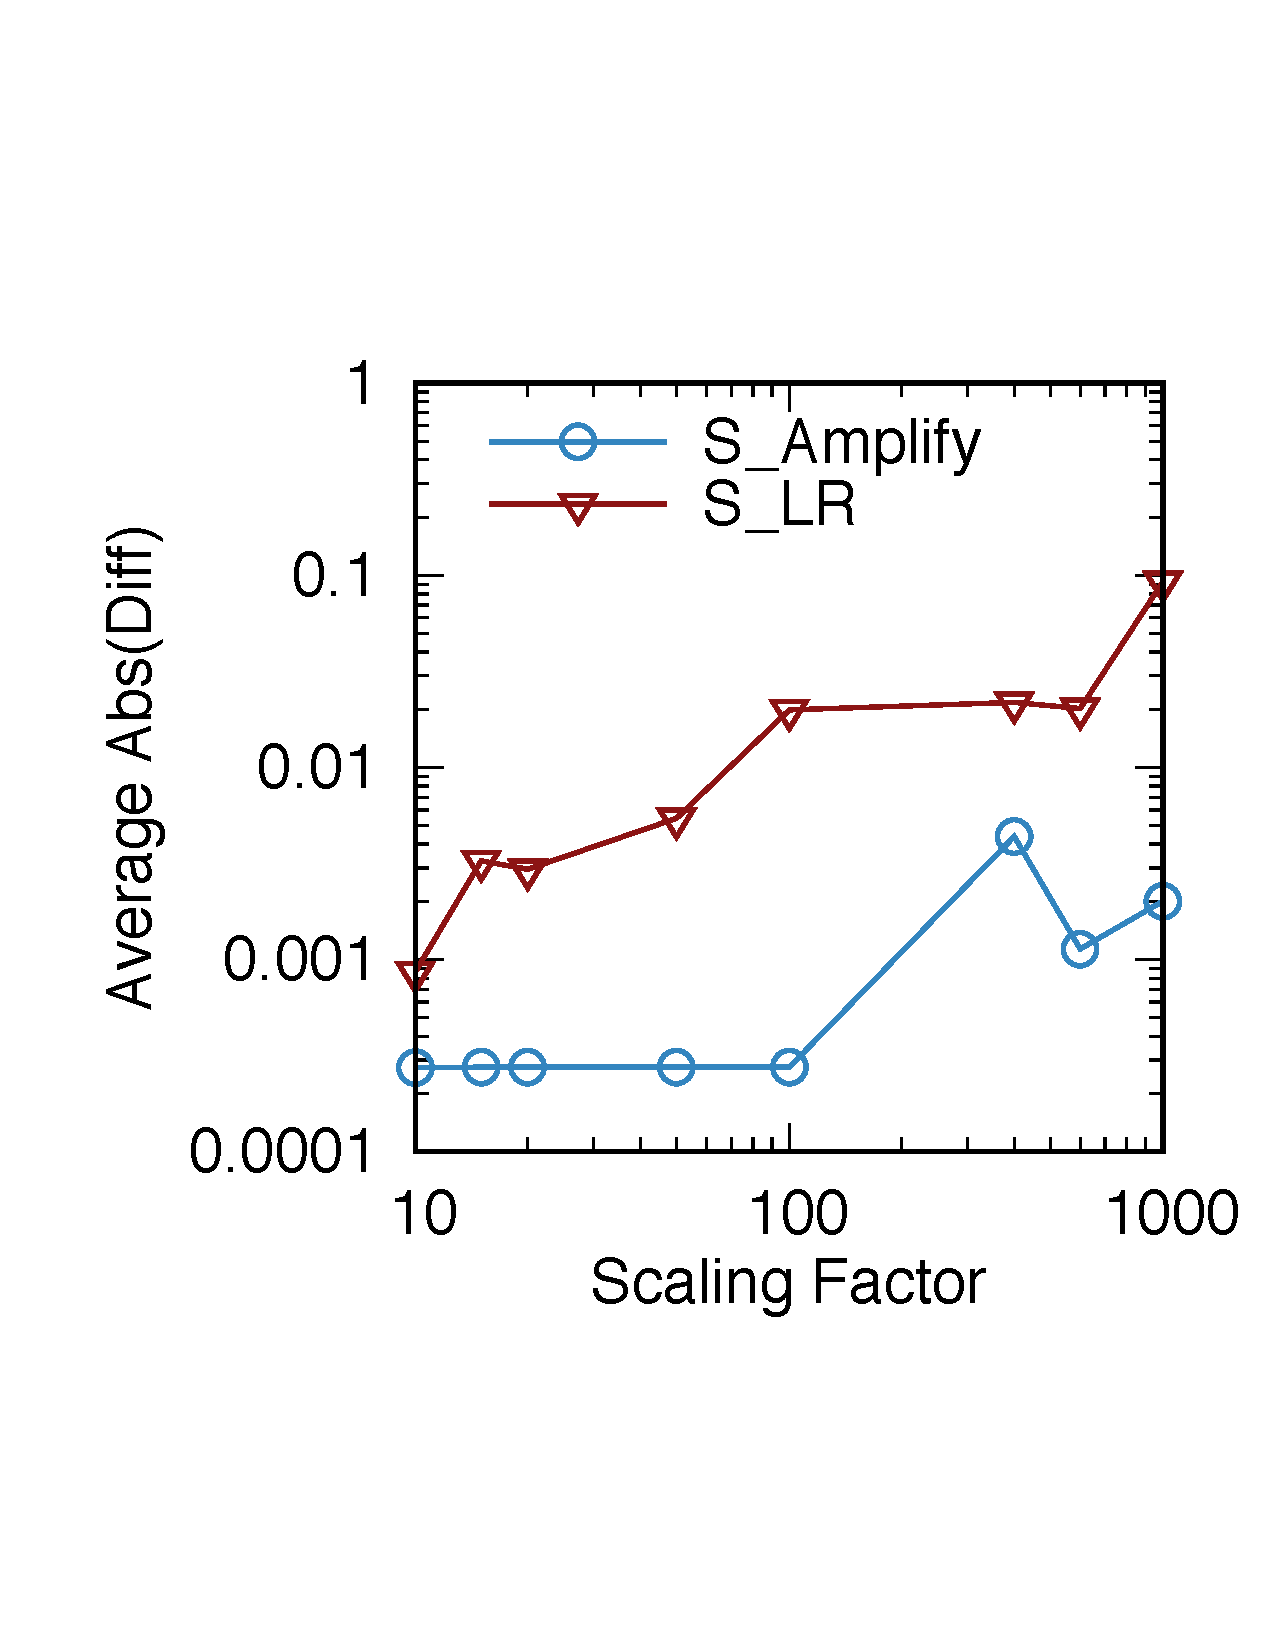
\includegraphics[width=.8\linewidth]{Graph/negSamp/AmplifyLRTheoryL1New.pdf}

		\captionof{figure}{Amplifying factor vs learning rate}
		\label{fig:amplifyLR}
	\end{minipage}%

\end{figure*}



% \begin{figure}[ht]
% 	\centering
% 	\begin{minipage}{.33\textwidth}
% 		\centering
% 		\captionsetup{justification=centering,margin=0.1cm}
% 		\includegraphics[width=.95\linewidth]{Graph/L2Theory_Step.pdf}
% 		\captionof{figure}{Model accuracy}
% 		\label{fig:l2Loss}
% 	\end{minipage}%
% 	\begin{minipage}{.33\textwidth}
% 		\centering
% 		\captionsetup{justification=centering,margin=0.1cm}
% 		\includegraphics[width=.95\linewidth]{Graph/theoryTime.pdf}
% 		\captionof{figure}{Training time.}
% 		\label{fig:trainingTime}
% 	\end{minipage}%
% 	\begin{minipage}{.33\textwidth}
% 		\captionsetup{justification=centering,margin=0.1cm}
% 		\centering
% 		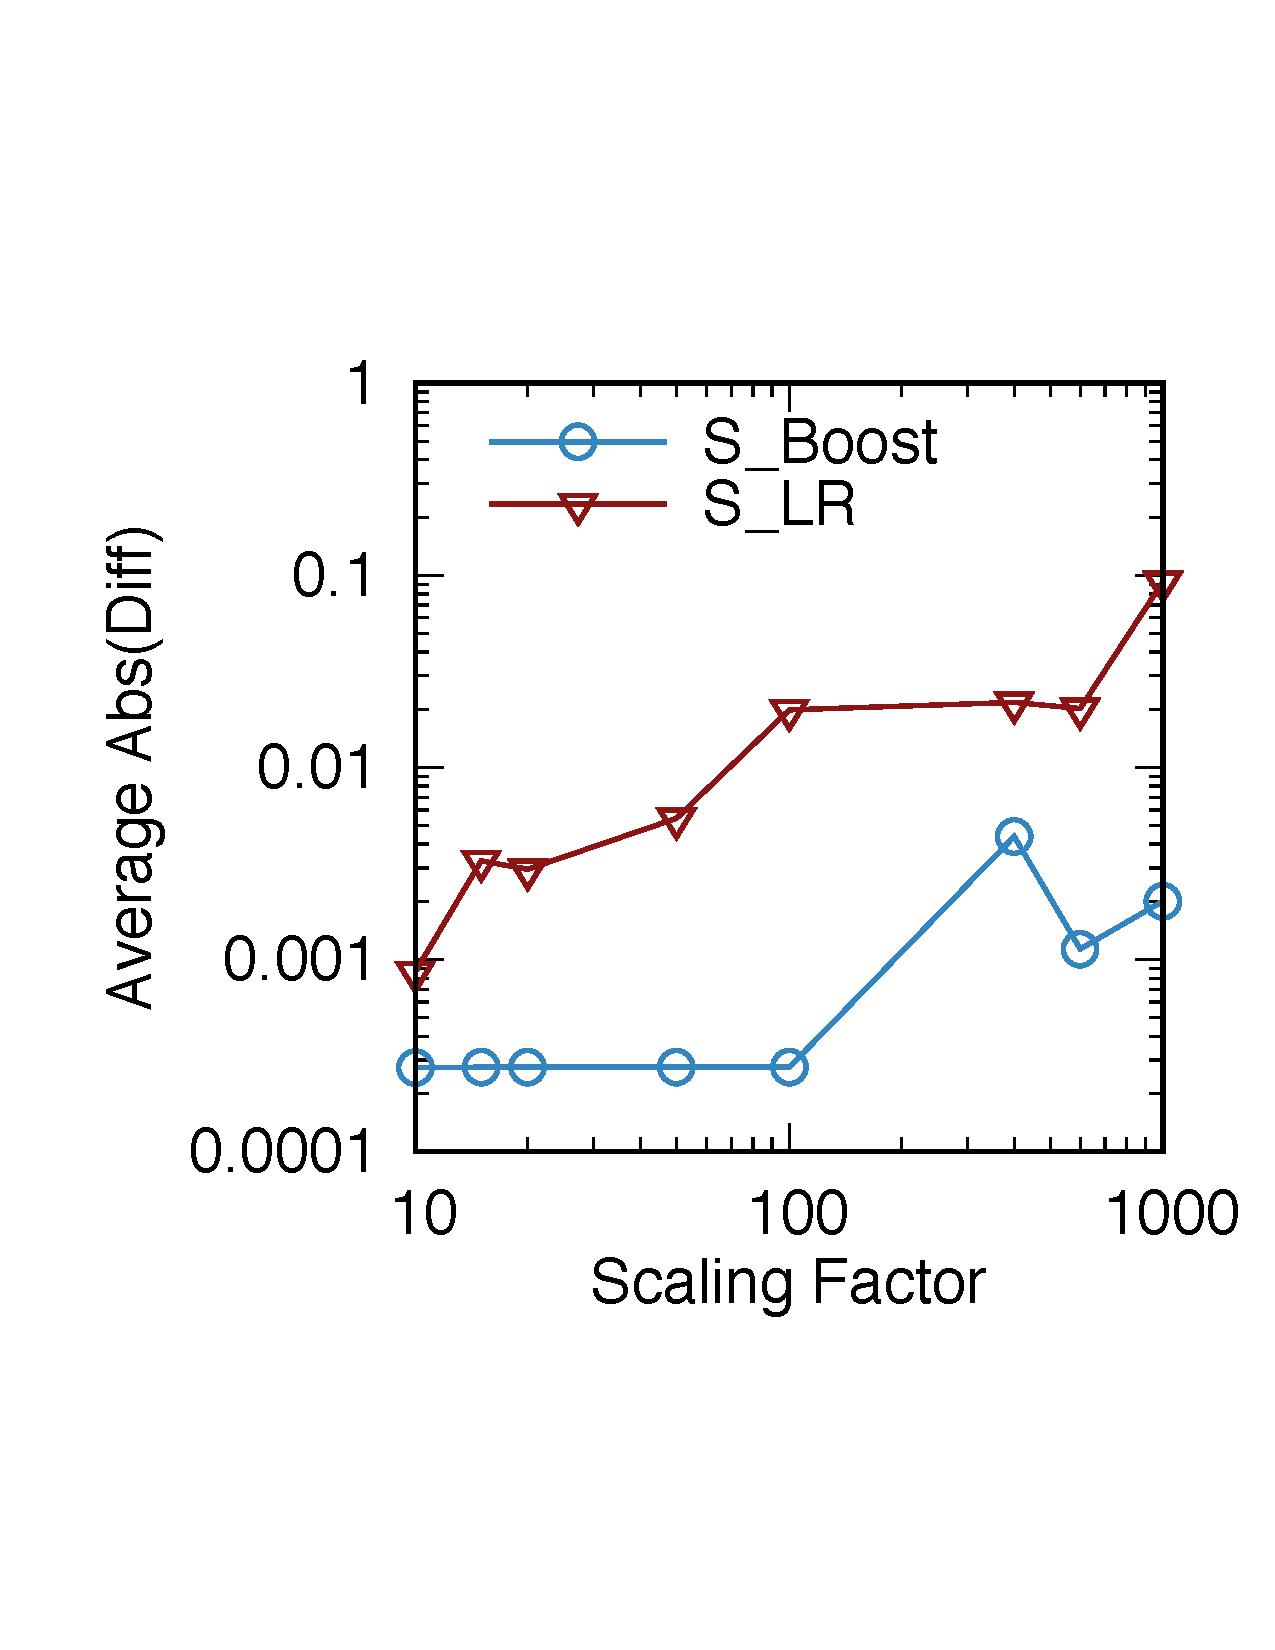
\includegraphics[width=.95\linewidth]{Graph/AmplifyLRTheoryL1New_1.pdf}
% 		\captionof{figure}{Amplifying factor vs learning rate}
% 		\label{fig:amplifyLR}
% 	\end{minipage}%
% 	%
% \end{figure}

\textbf{Model Accuracy and Convergence Rate.} 
In Figure~\ref{fig:l2Loss}, we compare the model accuracy and convergence rate when the model is trained with the four algorithms (FullGrad, Neg5, Neg5-Amplify3, Neg15) under the $L2$ loss function.\footnote{While we performed experiments under all three loss functions, we report the results only from $L2$ here due to space limit. The conclusions from other loss functions are essentially the same.} In the graph, the horizontal axis corresponds to the stochastic-gradient-descent training batch steps (with roughly 70 steps corresponding to one training epoch) and the vertical axis corresponds to the average absolute difference between the trained model $f_{\theta^*}(x, y)$ and MLE $\tilde{P}(y|x) = \frac{\#(x,y)}{\#(x)}$, i.e., $\sum_{(x,y)\in D} \frac{1}{\vert D\vert}\left\vert f_{\theta^*}(x, y) - \frac{\#(x,y)}{\#(x)}\right\vert$. 

From the graph, a few things are clear: (1) Full-gradient training converges to MLE. Even at epoch 1 (step 70), the mean absolute difference of \emph{FullGrad} is close to zero, indicating that it converged to MLE. (2) The amplifying factor $\beta$ effectively ``increases'' the negative sample size by the factor $\beta$ in terms of model accuracy. The mean absolute difference of Neg5-Amplify3 and Neg15 are the same at every training step --- they overlap so closely and it is difficult to tell them apart in the graph --- indicating that they both converge to the same model at the same rate. This result is what our theoretical analysis predicts: $(k=15, \beta = 1)$ leads to the same optimal model as $(k=5, \beta=3)$. (3) A model trained on larger $k$ approximates MLE better. The mean absolute difference of Neg15 is significantly smaller than that of Neg5. 

\textbf{Training Time and Computational Cost.} In Figure~\ref{fig:trainingTime}, we compare the training time of the four algorithms. The horizontal axis corresponds to training epochs and the vertical axis corresponds to training time, which roughly captures the computational cost of each algorithm. The vertical axis is logarithmic; since the training time of \emph{FullGrad} is two orders of magnitude larger than others, its result is not visible in the same graph otherwise. From the graph, we again observe what is predicted by our analysis. The training time of Neg5-Amplify3 is practically the same as that of Neg5. That is, Neg5-Amplify3 works almost like Neg5 in terms of its training time and computational cost, but it works almost like  Neg15 in terms of its model accuracy and convergence rate! Amplified negative sampling indeed gives the best of both worlds.

\textbf{Learning Rate vs Amplifying Factor.} In Figure~\ref{fig:amplifyLR}, we compare the effect of using different learning rates and amplifying factors. The graph is from training the model using Neg15 under $L1$ loss. The curve labeled as \emph{S\_LR} is obtained by multiplying the default learning rate of 0.025 by a factor between 10 and 1,000. The curve labeled as \emph{S\_Amplify} is obtained by including the amplifying factor $\beta$ between 10 and 1,000. The vertical axis is again in the logarithmic scale due to the high difference between the two curves and represents the model accuracy (the mean absolute difference from MLE) at the given learning rate/amplifying factor. From the graph, we see that changing the learning rate and changing the amplifying factor lead to vastly different results. As we increase the learning rate, the trained model diverges further away from MLE. When we increase the amplifying factor, however, the trained model stays close to MLE all the way through $\beta = 100$. Only after $\beta > 100$, the model starts to diverge and becomes unstable. This result is consistent with our analysis; according to Corollary~\ref{th:amplified}, amplifying converges to MLE at $\beta \approx 140$ under the current setting,\footnote{Amplified negative sampling converges to MLE when $\beta k p_y = 1$. Given $k=15$ and the uniform probability $p_y \approx 1/2000$ for this experiment, $\beta k p_y = 1$ at $\beta \approx 140$.} so its divergence beyond $\beta > 140$ is expected.

%\subsection{Language Model perplexity test}
%In this section, Amplified Negative Sampling method is tested on the Language Model on Penn Tree Bank(PTB) dataset~\citep{marcus-etal-1993-building} to demonstrate its performance. We use one of the commonly tested RNN Language model~\citep{zaremba2014recurrent} with the medium regularized settings as in ~\citep{blanc2017adaptive}. The PTB dataset contains 929K training words, 73k validation and 82k test words. We keep the original settings of the RNN model and set the hidden dimension as 650.
%
%The perplexity result is reported in Figure \ref{fig:neg5} and \ref{fig:neg15} for Neg5 and Neg15 experiment. For each negative sample setting, the amplifying factor is set to 1, 3 and 10 respectively. As the amplifying factor got enlarged, the perplexity got decreased. Every experiment converges in around 20 epochs.
%As shown in figure \ref{fig:neg5}, the amplifying factor can effectively decrease the perplexity compared with other model when only a few number of samples are allowed. Here the result is drawn from ~\citep{blanc2017adaptive} to demonstrate the Neg5 result with amplifying factor 10 can compete with ~\citep{blanc2017adaptive}'s 10 sample result.
%
%Further experiments are made on the effect of the amplifying factor. As shown in Figure \ref{fig:factor}, when the amplifying factor is increased from 1, the perplexity have a clear decrease until 10 and the perplexity starts to increase when the amplifying factor keeps enlarging. The best model performance will be obtained when the amplifying factor is configured around 10. An explanation based on formula (\ref{eq:amplifyed}) is the convergence condition is $t$(epoch) tends to infinity. However, in experiment, the training process will be stopped as the performance doesn't change anymore or the model got trapped in the saddle point. In this case, the model won't converge to the optimum value and a large amplifying factor will also change the convergence point to a non-optimum point.
%
%
%
%
%\begin{figure*}[ht]
%	\centering
%	\begin{minipage}{.31\textwidth}
%		\centering
%		\captionsetup{justification=centering,margin=0.1cm}
%		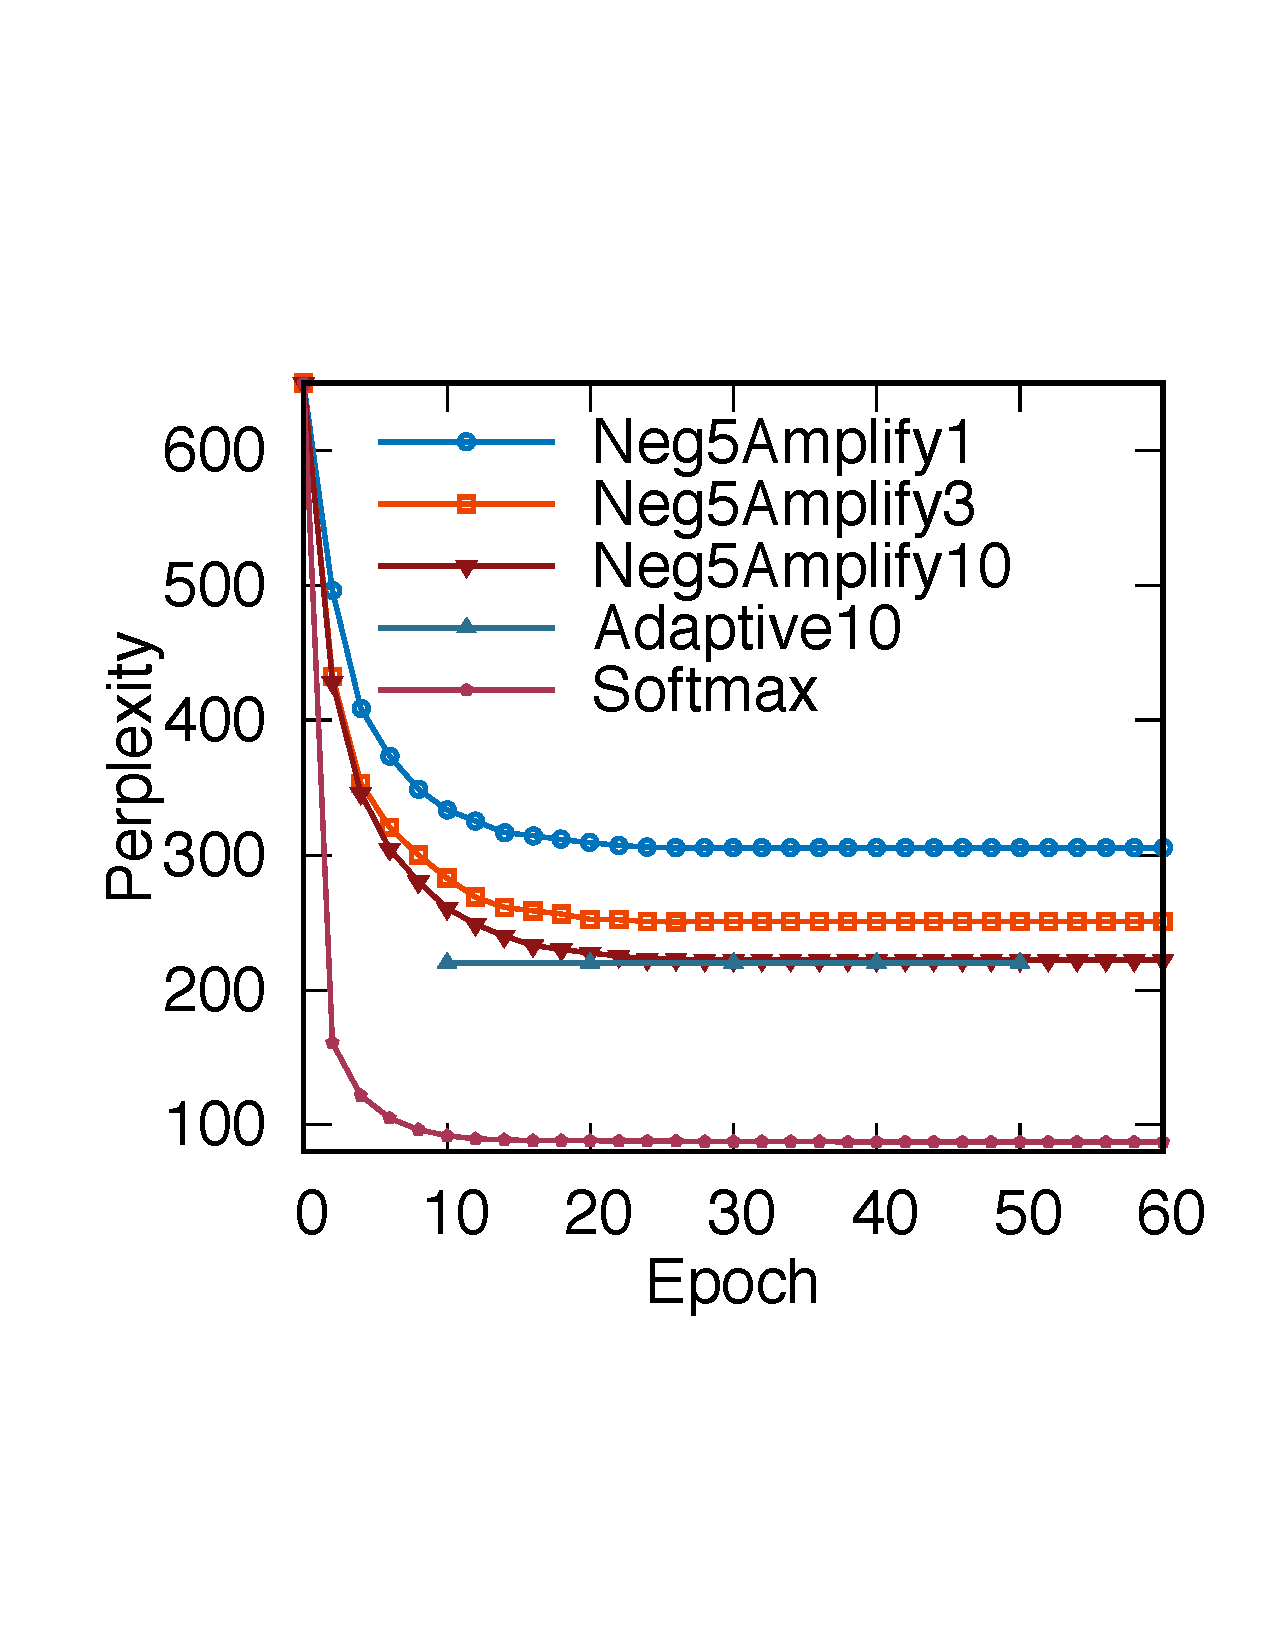
\includegraphics[width=1\linewidth]{Graph/negSamp/L2Neg5_60_Nolog.pdf}
%
%		\captionof{figure}{PTB: Negative sampling 5.}
%		\label{fig:neg5}
%	\end{minipage}%
%	\begin{minipage}{.31\textwidth}
%		\centering
%		\captionsetup{justification=centering,margin=0.1cm}
%		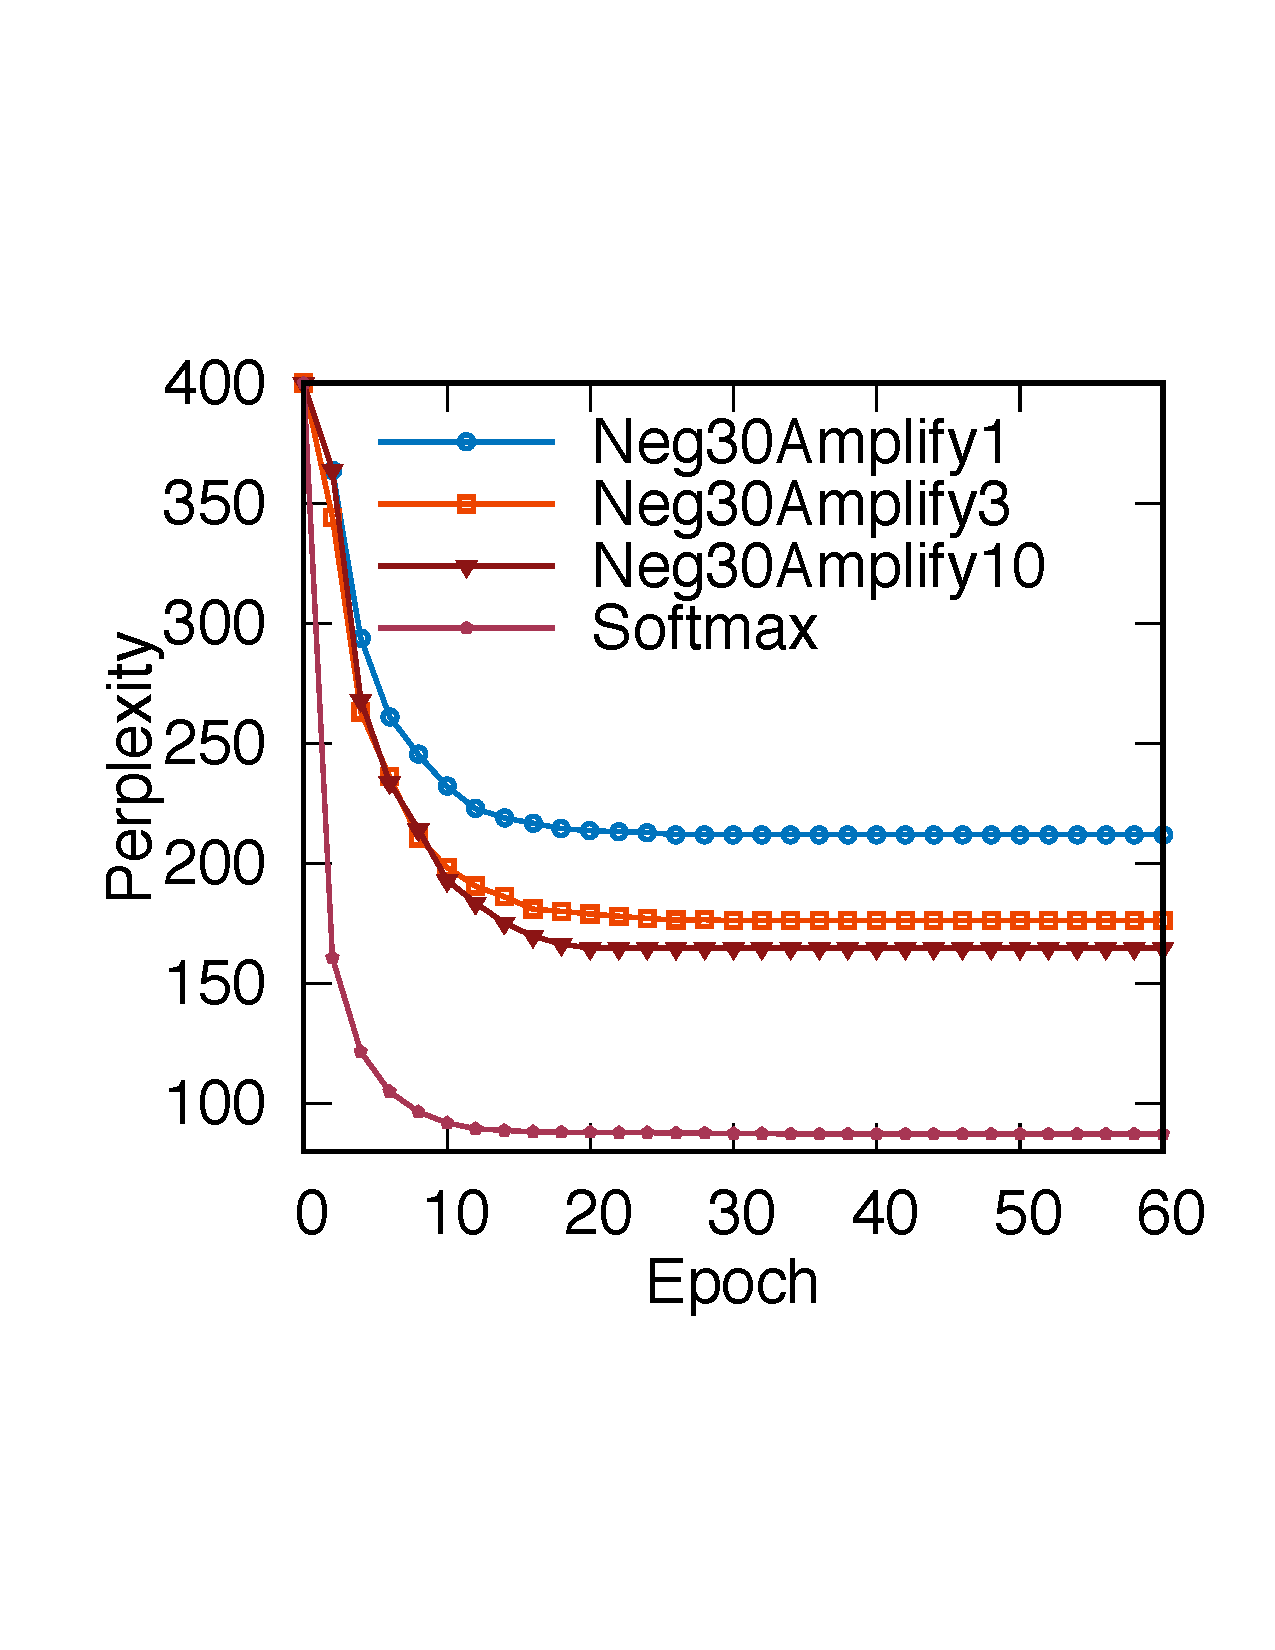
\includegraphics[width=1\linewidth]{Graph/negSamp/L2Neg30_60_Nolog.pdf}
%
%		\captionof{figure}{PTB: Negative sampling 15.}
%		\label{fig:neg15}
%	\end{minipage}%
%	\begin{minipage}{.38\textwidth}
%		\captionsetup{justification=centering,margin=0.1cm}
%		\centering
%		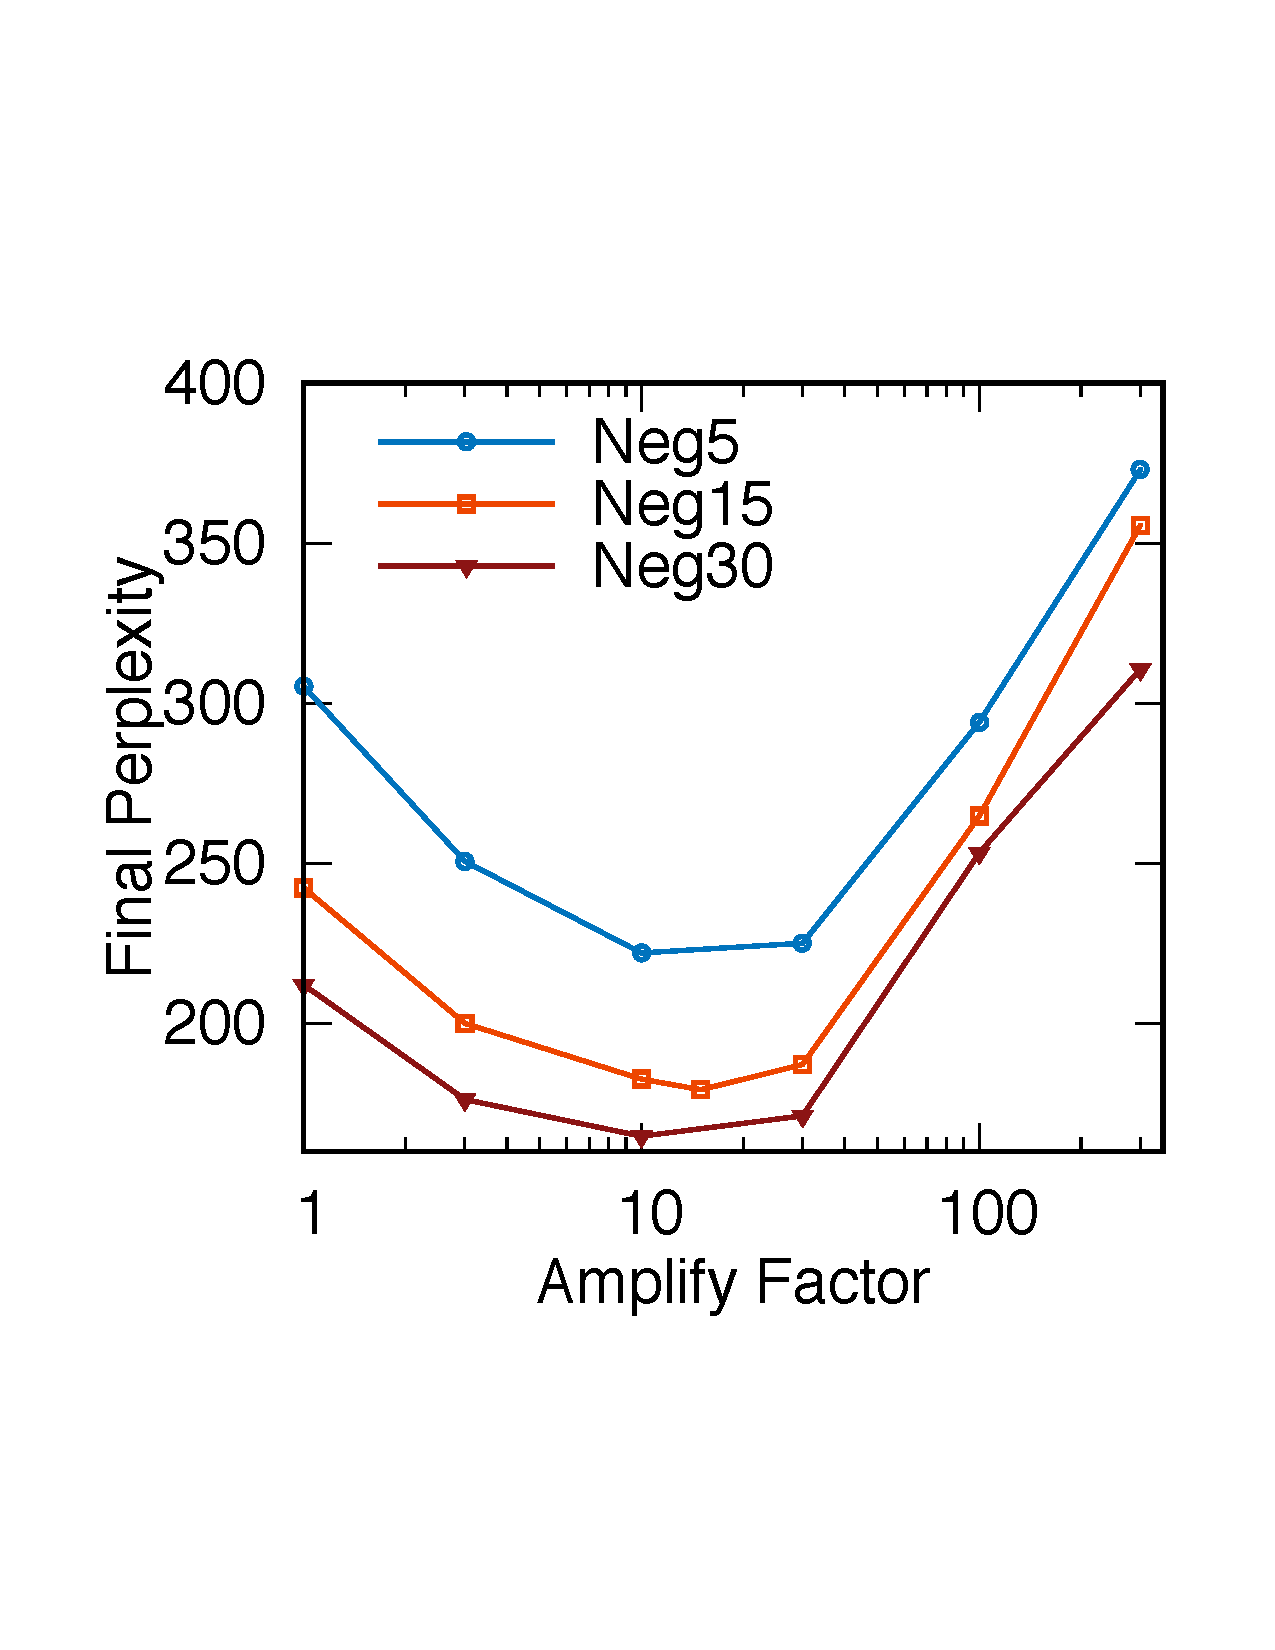
\includegraphics[width=.8\linewidth]{Graph/negSamp/L2NegAllAmplify.pdf}
%
%		\captionof{figure}{Different amplifying factor.}
%		\label{fig:factor}
%	\end{minipage}%
%
%\end{figure*}

\subsection{Experiments on Other Downstream Tasks}\label{sec:realworld}
In the previous set of experiments, we investigated the effect of amplified negative sampling on the trained model in terms of its difference from MLE. In the next set of experiments, we investigate its effect on three other downstream tasks: (a) word-analogy tasks (b) rare-word-similarity tasks and (c) graph-node-classification tasks. In all our experiments, we compare the results from Neg5, Neg5-Amplify3, and Neg15 at training epoch 3. 

\textbf{Word2vec: Word analogy.} This test is conducted with the CBOW model trained on the Text8 corpus~~\citep{mikolov2013distributed} using the code downloaded from ~\citep{word2vecGithub} after we add amplifying code. The performance is evaluated by the 14 word-analogy tasks in~~\citep{mikolov2013distributed}. We use the default parameter settings of the downloaded code.

\textbf{Fasttext: Rare word similarity.}
For the word-similarity task, we use the code for Fasttext ~\citep{fastText} downloaded from~~\citep{fastTextGithub} using its default settings after the addition of amplifying code. The model is trained on the rare word dataset (RW)~~\citep{luong2013better}. The effectiveness of a trained model is measured by the Spearman’s rank-correlation coefficient~~\citep{spearman1904proof} between the human judgment in the dataset and the output from the trained model.

\textbf{Node2vec: Node classification.} For the node classification task, we use the node2vec model ~\citep{node2vec-kdd2016} with the code downloaded from ~\citep{node2vecGithub}. The dataset used is BlogCatalog ~\citep{Zafarani+Liu:2009}. The nodes are embedded into a 50-dimensional space and we use 20-80 train-test split. The default parameter setting of the downloaded code is used after the addition of amplifying code.   

In Table~\ref{tbl:semantic} we show the accuracy of Neg5, Neg5-Amplify3, and Neg15 for the first 5 word-analogy semantic tasks of~~\citep{mikolov2013distributed}. From the results, the trend is clear: the performance of Neg5-Amplify3 is higher than Neg5 and is close to Neg15. In Table~\ref{tbl:time}, we show the training times of Word2vec, Fasttext, and Node2vec. In all three cases, the training time of Neg5-Amplify is close to Neg5 and is significantly smaller than that of Neg15. In the cases of Fasttext and Word2vec, the difference is by a factor 2. In the case of Node2vec, the difference is much smaller due to the dominance of other training overhead when the absolute training time is small.
From our other experiments whose results we could not include here due to space limit, we observe the same general trend: The downstream-task performance of Neg5-Amplify3 is close to Neg15 while its training cost is close to Neg5. 

\vspace{2em}
\makebox[\linewidth][c]{
\begin{minipage}{1\textwidth}
	%\begin{table}[h]
	
	\captionof{table}{Word-analogy semantic-task top-1 accuracy.}
	\label{tbl:semantic}
		\centering
		\begin{tabular}{| c |c c c|} 

			\hline
			Task Name & Neg5 & Neg5-Amplify3 & Neg15 \\
			\hline
			capital-common-countries & 38.14 & 43.02 & 47.43\\
			capital-world & 24.66 & 29.34 & 32.14\\
			city-in-state & 15.17 & 17.29 & 14.93\\
			currency & 15.72 & 22.26 & 22.21\\
			family & 56.86 & 60.30 & 64.27\\
			\hline
	\end{tabular}
\end{minipage}}
\vspace{2em}

% \begin{minipage}{.49\textwidth}
% %\begin{table}[h]

% \captionof{table}{Word-analogy semantic-task top-1 accuracy.}
% \label{tbl:semantic}
% \scalebox{0.8}{
%  \begin{tabular}{| c |c c c c c|} 
%  \hline

% Algorithm    &Task 1 & Task 2 & Task 3 & Task 4 & Task 5 \\
% \hline
% %  Neg5& 		37.15 &  23.21 &  14.55 &  16.42 &  52.94 \\

% %  Neg5-Amplify3& 42.29 &  27.2 &  14.18 &  22.02 &  58.5\\

% %  Neg15& 		47.04 &  31.47 &  16.04 &  22.15 &  65.69  \\
%  Neg5& 		38.14 &  24.66 &  15.17 &  15.72 &  56.86 \\

%  Neg5-Amplify3& 43.02 &  29.34 &  17.29 &  22.26 &  60.30\\

%  Neg15& 		47.43 &  32.14 &  14.93 &  22.21 &  64.27  \\


% \hline
% \end{tabular}}
% \vspace{3ex}
% 	\end{minipage}%
% 	\quad\quad%
% \begin{minipage}{0.49\textwidth}
%   \vspace{1.5ex}
% \captionof{table}{Mapping from Task ID to task real name for word analogy semantic-task.}
% \label{tbl:semanticName}
% \centering
% \scalebox{0.8}{
% \begin{tabular}{|c | c|} 
%  \hline

% Task ID & Real Name   \\
% \hline
% 1&	capital-common-countries\\
% 2&	capital-world\\
% 3&	city-in-state\\
% 4&	currency\\
% 5&	family\\
% % 6&	gram1-adjective-to-adverb\\
% % 7&	gram2-opposite\\
% % 8&	gram3-comparative\\
% % 9&	gram4-superlative\\
% % 10&	gram5-present-participle\\
% % 11&	gram6-nationality-adjective\\
% % 12&	gram7-past-tense\\
% % 13&	gram8-plural\\
% % 14&	gram9-plural-verbs\\

% \hline
% \end{tabular}}

% \end{minipage}

%\begin{minipage}{\textwidth}


\makebox[\linewidth][c]{
\begin{minipage}{1\textwidth}
	\captionof{table}{Training time (seconds).}
	\label{tbl:time}	
		\centering
		\begin{tabular}{|c|c c c|} 
		
			\hline
			Model & Neg5 &Neg5-Amplify3 & Neg15\\
			\hline
			Fasttext&736&731&1404\\
			Word2vec&17.35&17.37&36.93\\
			Node2vec&3.28&3.28 &4.00\\
			\hline
	\end{tabular}
	%   \captionof{table}{Training time (seconds).}
	% \label{tbl:time}
\end{minipage}}
%\end{minipage}
% \section{Experiments}\label{sec:experiments}
% The primary goal of this section is to experimentally investigate the following two issues: (1) Does the result of our analysis hold in practice? We want to examine how well our theoretical results match with experiments. We also want to experimentally explore a few questions raised in this chapter, including the choice of the optimal amplifying factor and the difference between the learning rate and the amplifying factor. (2) Does amplified negative sampling help other downstream tasks as well? The performance of other downstream tasks may not necessarily depend on how accurately the trained model captures the conditional probability $P(y|x)$, so we want to experimentally check whether amplified negative sampling has positive effects on other downstream tasks or not. 

% In the subsection (Model Accuracy and Training Efficiency)~\ref{sec:simulation}, we explore the first issue by measuring the difference between the maximum likelihood estimator (MLE) $\tilde{P}(y|x) = \frac{\#(x,y)}{\#(x)}$ and the models trained with (a) full-gradient training (b) negative sampling and (c) amplified negative sampling. The results of our experiments show that the conclusions of our analysis hold in practice to a surprising degree of accuracy. They also show that the learning rate and the amplifying factor have vastly different effects on the trained model. In the subsection (Experiments on Other Downstream Tasks)~\ref{sec:realworld}, we investigate the second issue by running experiments on three different downstream tasks: word-analogy tasks~~\citep{mikolov2013efficient}, rare-word-similarity tasks~~\citep{fastText}, and graph-node-classification tasks~~\citep{node2vec-kdd2016}. Here, we observe that amplified negative sampling leads to improved performance on these  downstream tasks as well. 


% In summary, our experimental results strongly indicate that there really is not much downside to using amplified negative sampling; as long as we use a reasonably small amplifying factor, say $\beta = 3$, amplified negative sampling leads to lower training time and higher model accuracy.

% \subsection{Model Accuracy and Training Efficiency}\label{sec:simulation}

% \textbf{Experimental Settings.} 
% In this subsection, we experimentally compare four training algorithms, full-gradient training (\textit{FullGrad}), 5 negative samples (\textit{Neg5}), 5 negative samples with the amplifying factor 3 (\textit{Neg5-Amplify3}), and 15 negative samples (\textit{Neg15}),
% under three different loss functions, $L1$, $L2$, and cross entropy. For the choice of the hypothesis space $f_{\theta}(x,y)$ and the training set, we use a setting similar to~~\citep{mikolov2013efficient}. That is, as our hypothesis space we use the skip-gram model of~~\citep{mikolov2013efficient} with a 100-dimensional hidden layer.
% As our dataset, we use a subset of Text8 corpus from~~\citep{mikolov2013efficient} by extracting the first 75,000 words and applying the same min\_count filter of 5 in~~\citep{mikolov2013efficient}.\footnote{Using a subset of Text8 here is due to the high training cost of \textit{FullGrad} and our desire to keep the training time at a manageable level. In our next experiments on other downstream tasks, we run report our results from experiments on much larger datasets.} We use the stochastic-gradient descent (SGD) with the batch size of 500 as the training algorithm. All our experiments use the window size 3 and the learning rate 0.025 unless noted otherwise. All other parameter settings are the same as in~~\citep{mikolov2013efficient}. All results reported are the average of three independent runs with identical settings. All codes were implemented using PyTorch v1.0.1. 

% \begin{figure*}[ht]
% 	\centering
% 	\begin{minipage}{.31\textwidth}
% 		\centering
% 		\captionsetup{justification=centering,margin=0.1cm}
% 		\includegraphics[width=1\linewidth]{Graph/L2Theory_Step.pdf}
% 		\vspace{-13ex}
% 		\captionof{figure}{Model accuracy.}
% 		\label{fig:l2Loss}
% 	\end{minipage}%
% 	\begin{minipage}{.31\textwidth}
% 		\centering
% 		\captionsetup{justification=centering,margin=0.1cm}
% 		\includegraphics[width=1\linewidth]{Graph/theoryTime.pdf}
% 		\vspace{-13ex}
% 		\captionof{figure}{Training time.}
% 		\label{fig:trainingTime}
% 	\end{minipage}%
% 	\begin{minipage}{.38\textwidth}
% 		\captionsetup{justification=centering,margin=0.1cm}
% 		\centering
% 		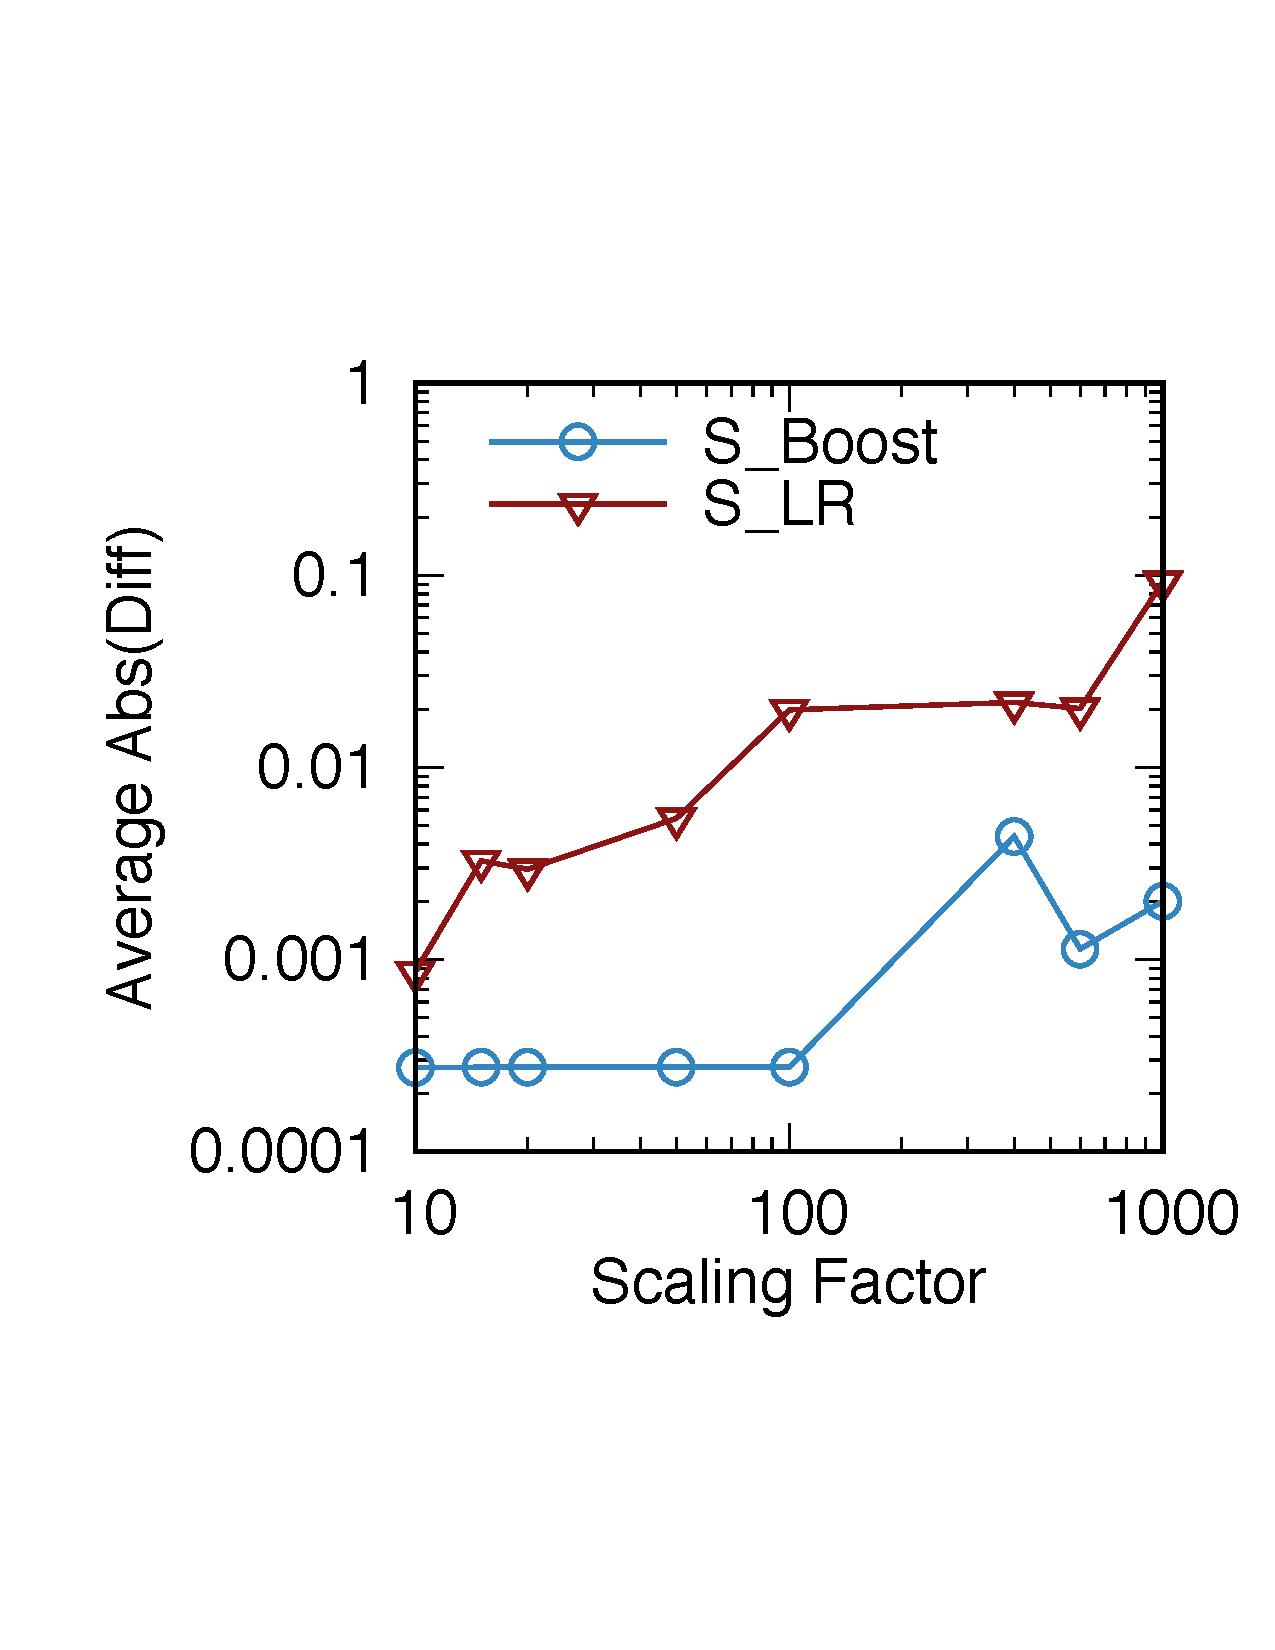
\includegraphics[width=.8\linewidth]{Graph/AmplifyLRTheoryL1New_1.pdf}
% 		\vspace{-10ex}
% 		\captionof{figure}{Amplifying factor vs learning rate.}
% 		\label{fig:amplifyLR}
% 	\end{minipage}%
% 	\vspace{-1.5em}
% \end{figure*}



% % \begin{figure}[ht]
% % 	\centering
% % 	\begin{minipage}{.33\textwidth}
% % 		\centering
% % 		\captionsetup{justification=centering,margin=0.1cm}
% % 		\includegraphics[width=.95\linewidth]{Graph/L2Theory_Step.pdf}
% % 		\captionof{figure}{Model accuracy}
% % 		\label{fig:l2Loss}
% % 	\end{minipage}%
% % 	\begin{minipage}{.33\textwidth}
% % 		\centering
% % 		\captionsetup{justification=centering,margin=0.1cm}
% % 		\includegraphics[width=.95\linewidth]{Graph/theoryTime.pdf}
% % 		\captionof{figure}{Training time.}
% % 		\label{fig:trainingTime}
% % 	\end{minipage}%
% % 	\begin{minipage}{.33\textwidth}
% % 		\captionsetup{justification=centering,margin=0.1cm}
% % 		\centering
% % 		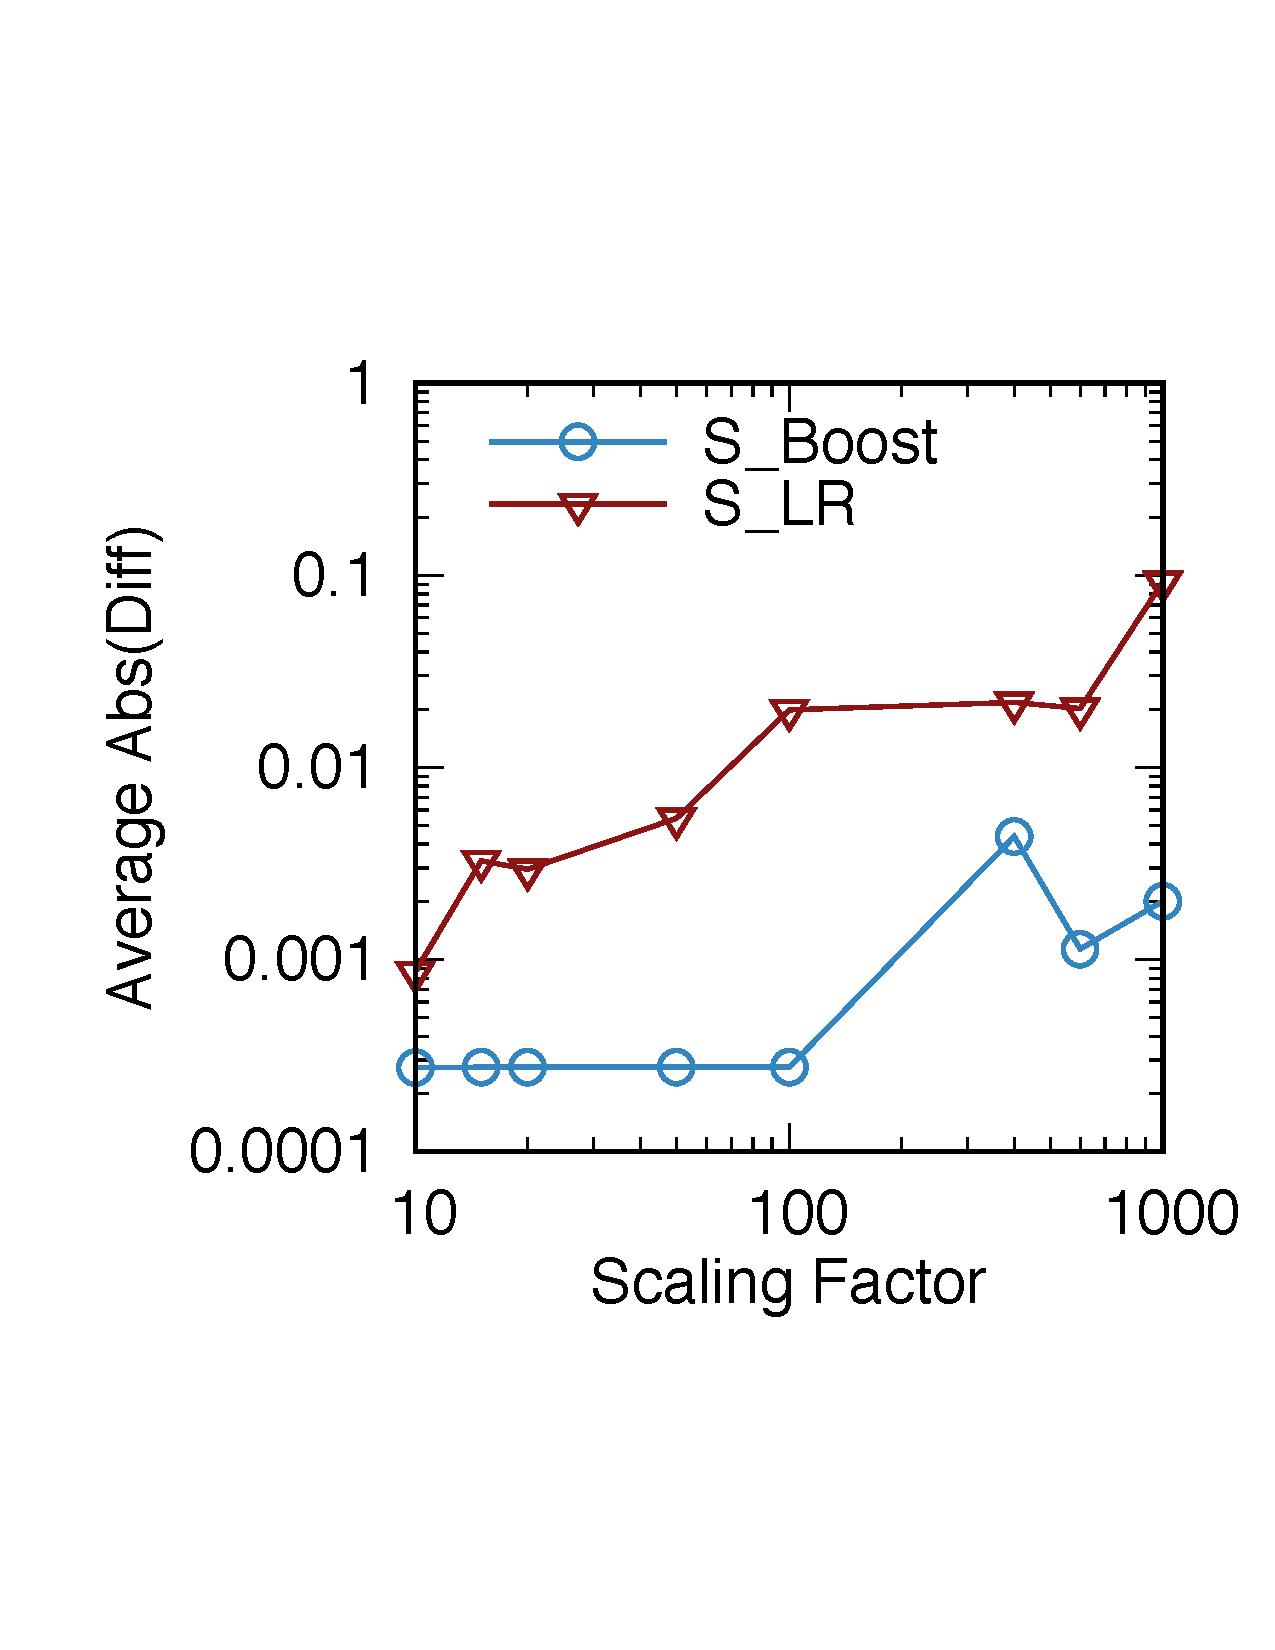
\includegraphics[width=.95\linewidth]{Graph/AmplifyLRTheoryL1New_1.pdf}
% % 		\captionof{figure}{Amplifying factor vs learning rate}
% % 		\label{fig:amplifyLR}
% % 	\end{minipage}%
% % 	%
% % \end{figure}

% \textbf{Model Accuracy and Convergence Rate.} 
% In Figure~\ref{fig:l2Loss}, we compare the model accuracy and convergence rate when the model is trained with the four algorithms (FullGrad, Neg5, Neg5-Amplify3, Neg15) under the $L2$ loss function.\footnote{While we performed experiments under all three loss functions, we report the results only from $L2$ here due to space limit. The conclusions from other loss functions are essentially the same.} In the graph, the horizontal axis corresponds to the stochastic-gradient-descent training batch steps (with roughly 70 steps corresponding to one training epoch) and the vertical axis corresponds to the average absolute difference between the trained model $f_{\theta^*}(x, y)$ and MLE $\tilde{P}(y|x) = \frac{\#(x,y)}{\#(x)}$, i.e., $\sum_{(x,y)\in D} \frac{1}{\vert D\vert}\left\vert f_{\theta^*}(x, y) - \frac{\#(x,y)}{\#(x)}\right\vert$. 

% From the graph, a few things are clear: (1) Full-gradient training converges to MLE. Even at epoch 1 (step 70), the mean absolute difference of \emph{FullGrad} is close to zero, indicating that it converged to MLE. (2) The amplifying factor $\beta$ effectively ``increases'' the negative sample size by the factor $\beta$ in terms of model accuracy. The mean absolute difference of Neg5-Amplify3 and Neg15 are the same at every training step --- they overlap so closely and it is difficult to tell them apart in the graph --- indicating that they both converge to the same model at the same rate. This result is what our theoretical analysis predicts: $(k=15, \beta = 1)$ leads to the same optimal model as $(k=5, \beta=3)$. (3) A model trained on larger $k$ approximates MLE better. The mean absolute difference of Neg15 is significantly smaller than that of Neg5. 

% \textbf{Training Time and Computational Cost.} In Figure~\ref{fig:trainingTime}, we compare the training time of the four algorithms. The horizontal axis corresponds to training epochs and the vertical axis corresponds to training time, which roughly captures the computational cost of each algorithm. The vertical axis is logarithmic; since the training time of \emph{FullGrad} is two orders of magnitude larger than others, its result is not visible in the same graph otherwise. From the graph, we again observe what is predicted by our analysis. The training time of Neg5-Amplify3 is practically the same as that of Neg5. That is, Neg5-Amplify3 works almost like Neg5 in terms of its training time and computational cost, but it works almost like  Neg15 in terms of its model accuracy and convergence rate! Amplified negative sampling indeed gives the best of both worlds.

% \textbf{Learning Rate vs Amplifying Factor.} In Figure~\ref{fig:amplifyLR}, we compare the effect of using different learning rates and amplifying factors. The graph is from training the model using Neg15 under $L1$ loss. The curve labeled as \emph{S\_LR} is obtained by multiplying the default learning rate of 0.025 by a factor between 10 and 1,000. The curve labeled as \emph{S\_Amplify} is obtained by including the amplifying factor $\beta$ between 10 and 1,000. The vertical axis is again in the logarithmic scale due to the high difference between the two curves and represents the model accuracy (the mean absolute difference from MLE) at the given learning rate/amplifying factor. From the graph, we see that changing the learning rate and changing the amplifying factor lead to vastly different results. As we increase the learning rate, the trained model diverges further away from MLE. When we increase the amplifying factor, however, the trained model stays close to MLE all the way through $\beta = 100$. Only after $\beta > 100$, the model starts to diverge and becomes unstable. This result is consistent with our analysis; according to Corollary~\ref{th:amplified}, amplifying converges to MLE at $\beta \approx 140$ under the current setting,\footnote{Amplified negative sampling converges to MLE when $\beta k p_y = 1$. Given $k=15$ and the uniform probability $p_y \approx 1/2000$ for this experiment, $\beta k p_y = 1$ at $\beta \approx 140$.} so its divergence beyond $\beta > 140$ is expected.

% \subsection{Experiments on Other Downstream Tasks}\label{sec:realworld}
% In the previous set of experiments, we investigated the effect of amplified negative sampling on the trained model in terms of its difference from MLE. In the next set of experiments, we investigate its effect on three other downstream tasks: (a) word-analogy tasks (b) rare-word-similarity tasks and (c) graph-node-classification tasks. In all our experiments, we compare the results from Neg5, Neg5-Amplify3, and Neg15 at training epoch 3. 

% \textbf{Word2vec: Word analogy.} This test is conducted with the CBOW model trained on the Text8 corpus~~\citep{mikolov2013distributed} using the code downloaded from ~\citep{word2vecGithub} after we add amplifying code. The performance is evaluated by the 14 word-analogy tasks in~~\citep{mikolov2013distributed}. We use the default parameter settings of the downloaded code.

% \textbf{Fasttext: Rare word similarity.}
% For the word-similarity task, we use the code for Fasttext ~\citep{fastText} downloaded from~~\citep{fastTextGithub} using its default settings after the addition of amplifying code. The model is trained on the rare word dataset (RW)~~\citep{luong2013better}. The effectiveness of a trained model is measured by the Spearman’s rank-correlation coefficient~~\citep{spearman1904proof} between the human judgment in the dataset and the output from the trained model.

% \textbf{Node2vec: Node classification.} For the node classification task, we use the node2vec model ~\citep{node2vec-kdd2016} with the code downloaded from ~\citep{node2vecGithub}. The dataset used is BlogCatalog ~\citep{Zafarani+Liu:2009}. The nodes are embedded into a 50-dimensional space and we use 20-80 train-test split. The default parameter setting of the downloaded code is used after the addition of amplifying code.   

%  In Table~\ref{tbl:semantic} we show the accuracy of Neg5, Neg5-Amplify3, and Neg15 for the first 5 word-analogy semantic tasks of~~\citep{mikolov2013distributed}. From the results, the trend is clear: the performance of Neg5-Amplify3 is higher than Neg5 and is close to Neg15. As shown in Figure~\ref{fig:wordAnaTask}, a detailed analysis to one word analogy task by epochs, performance improvement is more obvious under low epochs. With more iterations, the Neg5 gets sufficient training and can be accurate enough. 

%  In Table~\ref{tbl:time}, we show the training times of Word2vec, Fasttext, and Node2vec. In all three cases, the training time of Neg5-Amplify is close to Neg5 and is significantly smaller than that of Neg15. In the cases of Fasttext and Word2vec, the difference is by a factor 2. In the case of Node2vec, the difference is much smaller due to the dominance of other training overhead when the absolute training time is small.
% %  From our other experiments whose results we could not include here due to space limit,

%  From our other experiments as shown in Figure~\ref{fig:fastTextSimilarWord} and ~\ref{fig:nodeClassification},
%  we observe the same general trend: the downstream-task performance of Neg5-Amplify3 is close to Neg15 while its training cost is close to Neg5. The improvements are more signification for the first several iterations.


%  \begin{figure*}[ht]
% 	\centering
% 	\begin{minipage}{.31\textwidth}
% 		\centering
% 		\captionsetup{justification=centering,margin=0.1cm}
% 		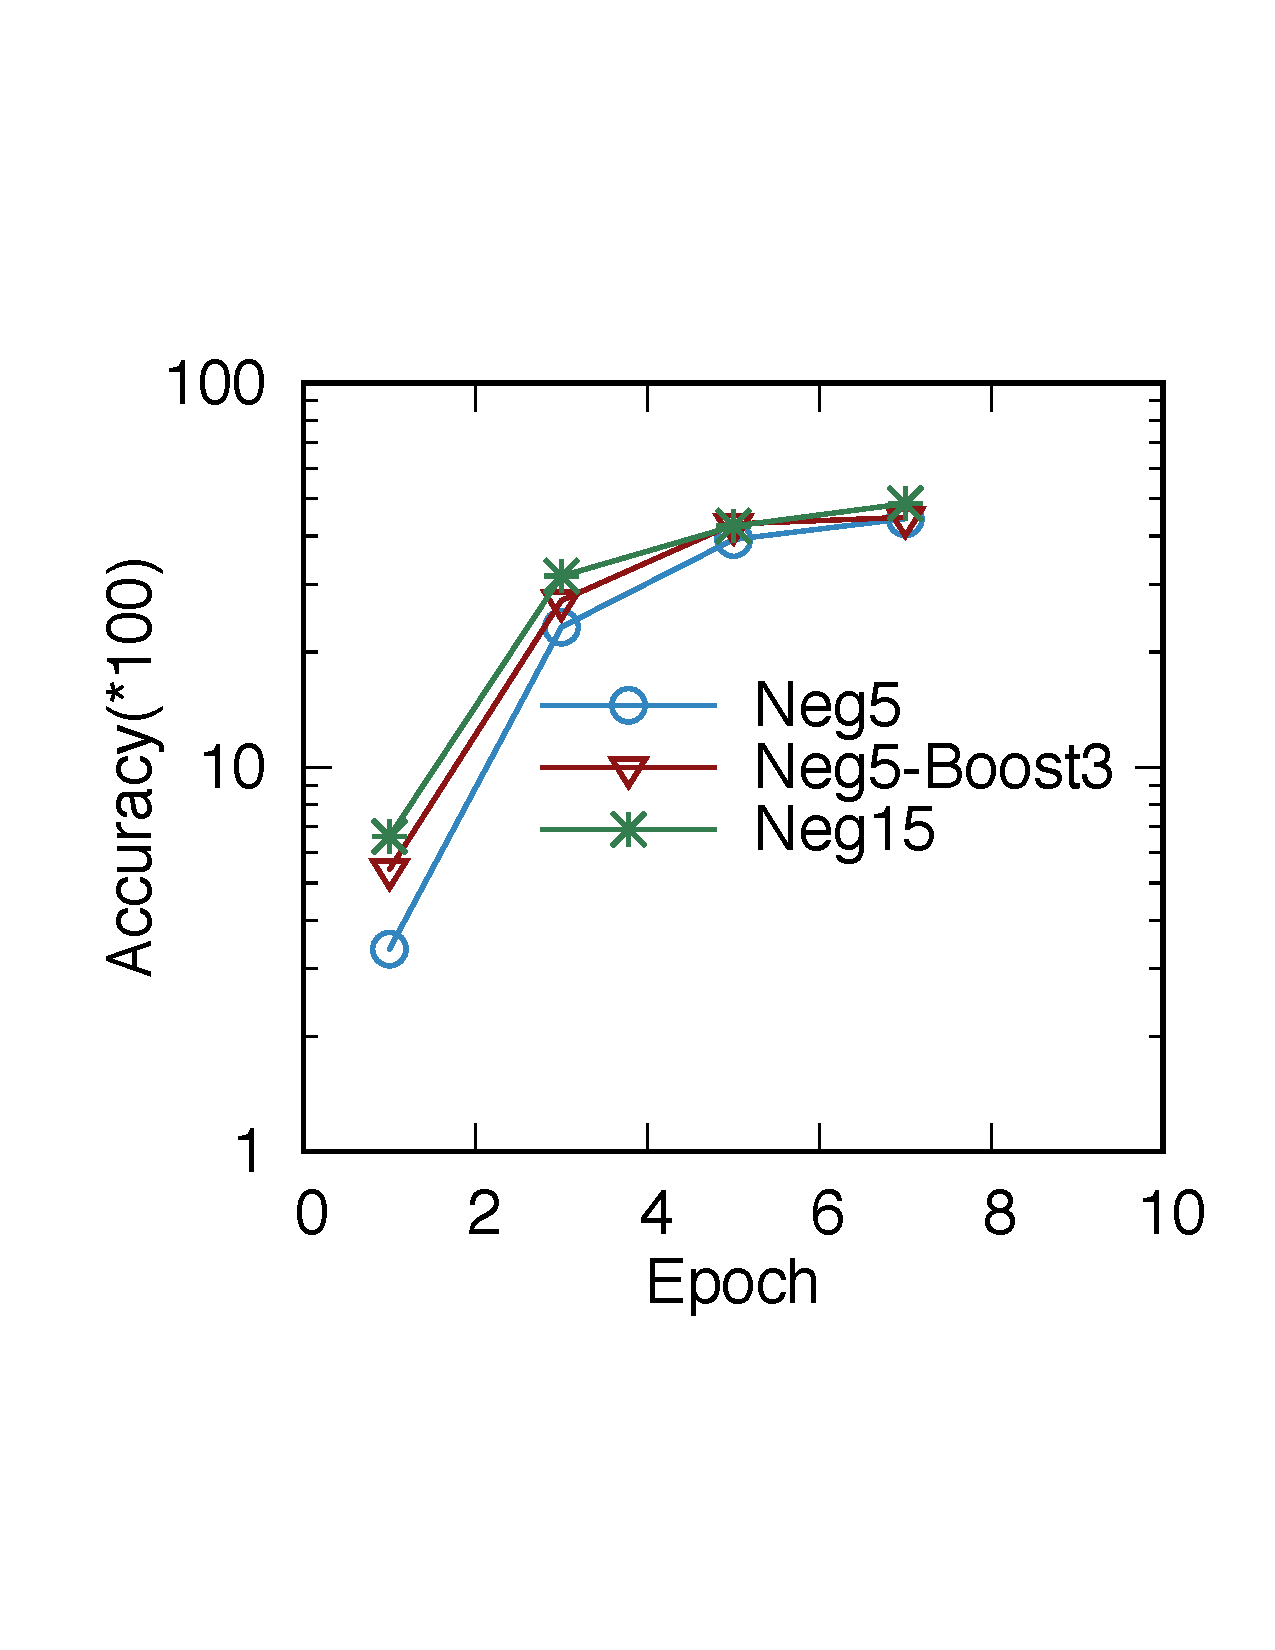
\includegraphics[width=1\linewidth]{Graph/negSamp/word2vecTask1.pdf}
% 		\vspace{-13ex}
% 		\captionof{figure}{Word analogy task: capital-common-countries.}
% 		\label{fig:wordAnaTask}
% 	\end{minipage}%
% 	\begin{minipage}{.31\textwidth}
% 		\centering
% 		\captionsetup{justification=centering,margin=0.1cm}
% 		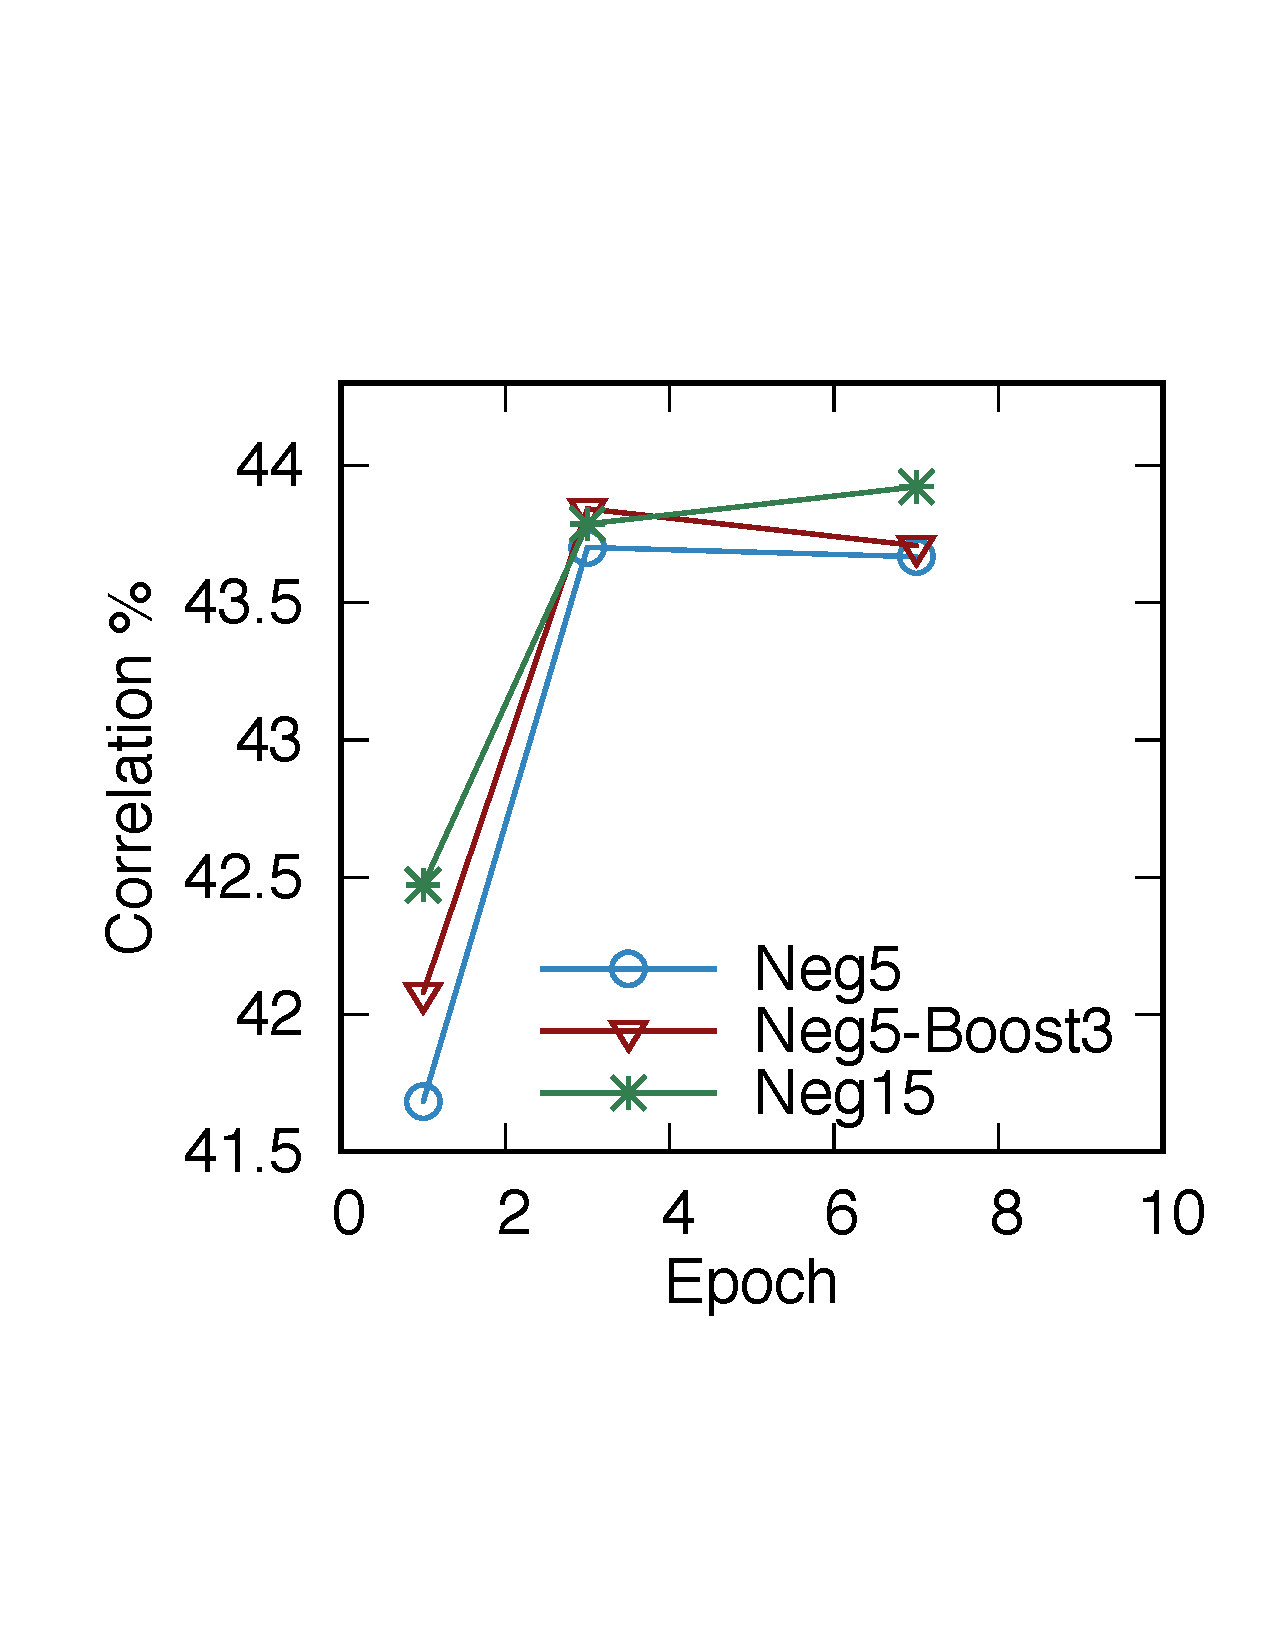
\includegraphics[width=1\linewidth]{Graph/negSamp/fasttext.pdf}
% 		\vspace{-13ex}
% 		\captionof{figure}{Fasttext: rare word's similarity.}
% 		\label{fig:fastTextSimilarWord}
% 	\end{minipage}%
% 	\begin{minipage}{.38\textwidth}
% 		\captionsetup{justification=centering,margin=0.1cm}
% 		\centering
% 		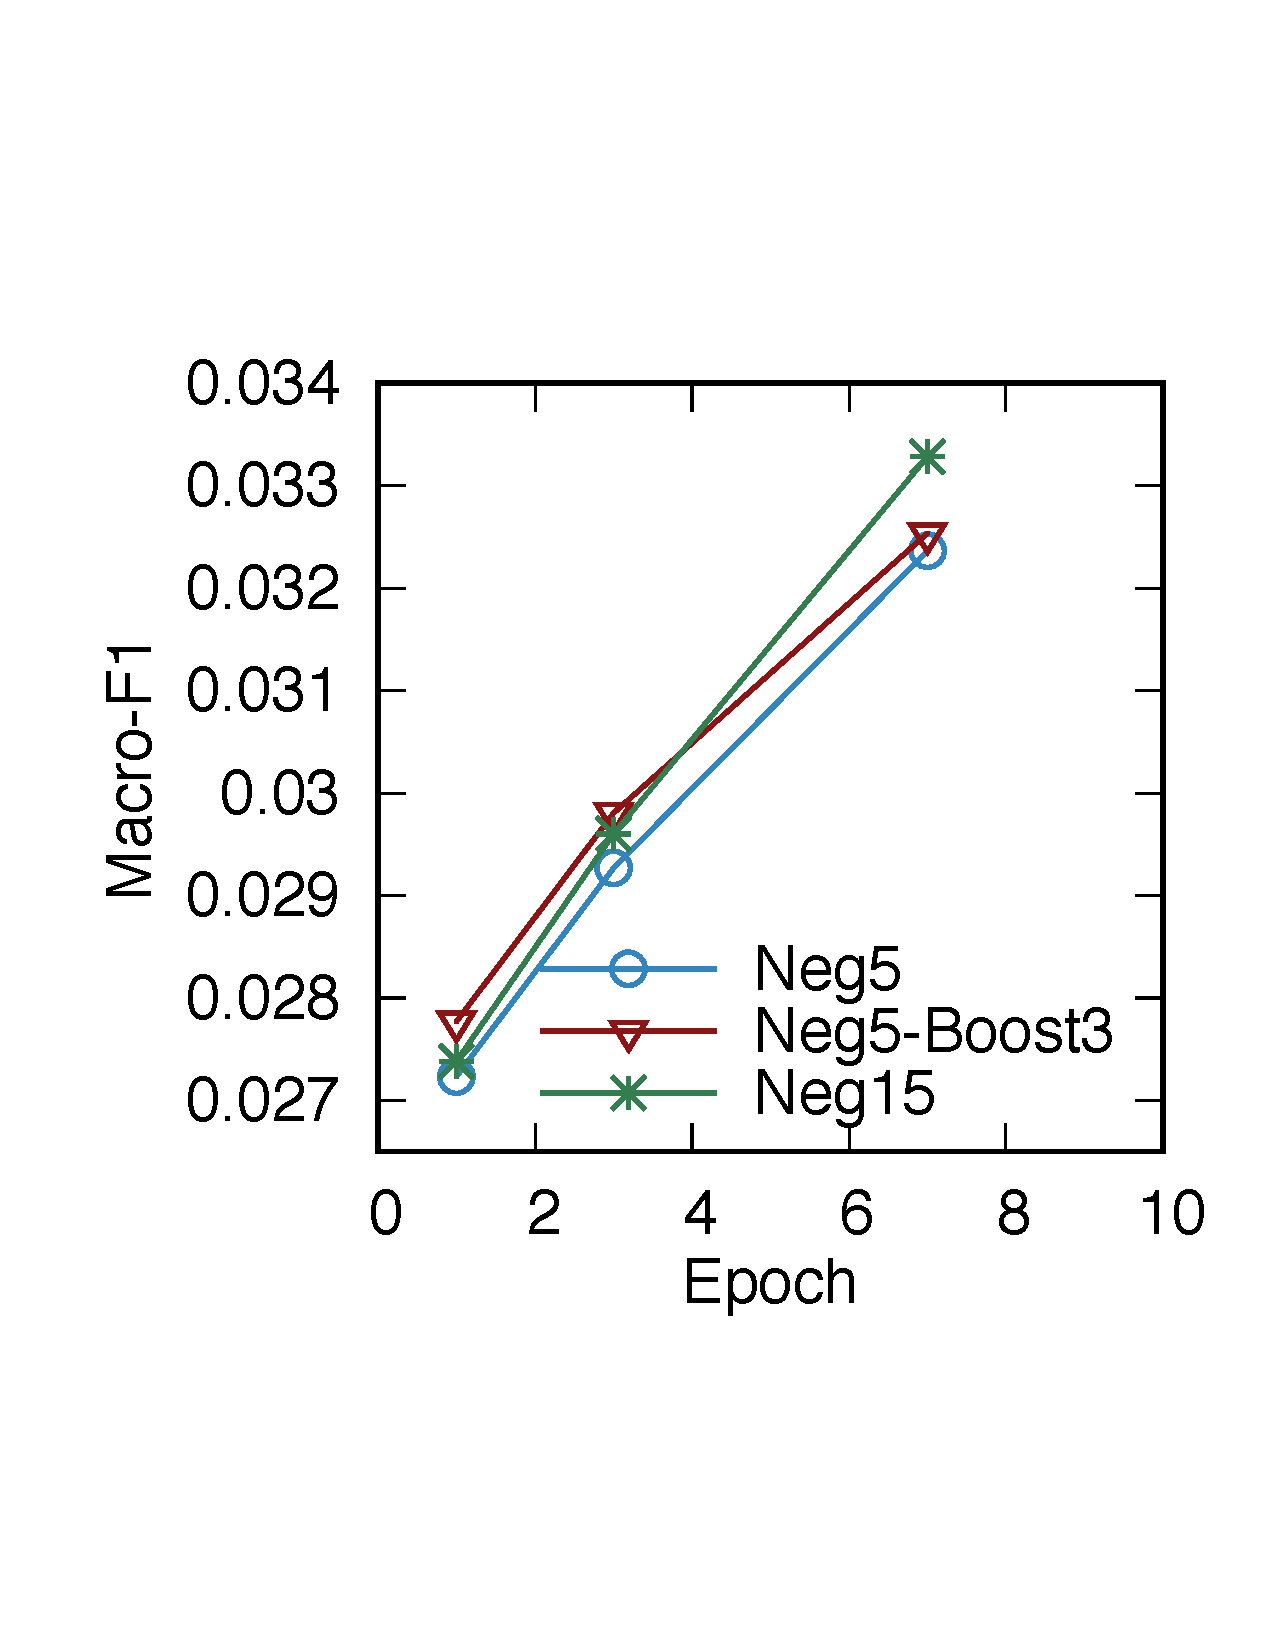
\includegraphics[width=.8\linewidth]{Graph/negSamp/node2vec.pdf}
% 		\vspace{-10ex}
% 		\captionof{figure}{Node classification.}
% 		\label{fig:nodeClassification}
% 	\end{minipage}%
% 	\vspace{-1.5em}
% \end{figure*}


% \begin{minipage}{.49\textwidth}
% %\begin{table}[h]
% \centering
%  \vspace{1.5ex}
% \captionof{table}{Word-analogy semantic-task top-1 accuracy.}
% \label{tbl:semantic}
% \scalebox{0.8}{
%  \begin{tabular}{| c |c c c|} 
%  \hline
% Task Name & Neg5 & Neg5-Amplify3 & Neg15 \\
% \hline
% capital-common-countries & 38.14 & 43.02 & \textbf{47.43}\\
% capital-world & 24.66 & 29.34 & \textbf{32.14}\\
% city-in-state & 15.17 & \textbf{17.29} & 14.93\\
% currency & 15.72 & \textbf{22.26} & 22.21\\
% family & 56.86 & 60.30 & \textbf{64.27}\\


% \hline
% \end{tabular}}
% \end{minipage}


% % \begin{minipage}{.49\textwidth}
% % %\begin{table}[h]

% % \captionof{table}{Word-analogy semantic-task top-1 accuracy.}
% % \label{tbl:semantic}
% % \scalebox{0.8}{
% %  \begin{tabular}{| c |c c c c c|} 
% %  \hline

% % Algorithm    &Task 1 & Task 2 & Task 3 & Task 4 & Task 5 \\
% % \hline
% % %  Neg5& 		37.15 &  23.21 &  14.55 &  16.42 &  52.94 \\

% % %  Neg5-Amplify3& 42.29 &  27.2 &  14.18 &  22.02 &  58.5\\

% % %  Neg15& 		47.04 &  31.47 &  16.04 &  22.15 &  65.69  \\
% %  Neg5& 		38.14 &  24.66 &  15.17 &  15.72 &  56.86 \\

% %  Neg5-Amplify3& 43.02 &  29.34 &  17.29 &  22.26 &  60.30\\

% %  Neg15& 		47.43 &  32.14 &  14.93 &  22.21 &  64.27  \\


% % \hline
% % \end{tabular}}
% % \vspace{3ex}
% % 	\end{minipage}%
% % 	\quad\quad%
% % \begin{minipage}{0.49\textwidth}
% %   \vspace{1.5ex}
% % \captionof{table}{Mapping from Task ID to task real name for word analogy semantic-task.}
% % \label{tbl:semanticName}
% % \centering
% % \scalebox{0.8}{
% % \begin{tabular}{|c | c|} 
% %  \hline

% % Task ID & Real Name   \\
% % \hline
% % 1&	capital-common-countries\\
% % 2&	capital-world\\
% % 3&	city-in-state\\
% % 4&	currency\\
% % 5&	family\\
% % % 6&	gram1-adjective-to-adverb\\
% % % 7&	gram2-opposite\\
% % % 8&	gram3-comparative\\
% % % 9&	gram4-superlative\\
% % % 10&	gram5-present-participle\\
% % % 11&	gram6-nationality-adjective\\
% % % 12&	gram7-past-tense\\
% % % 13&	gram8-plural\\
% % % 14&	gram9-plural-verbs\\

% % \hline
% % \end{tabular}}

% % \end{minipage}

% %\begin{minipage}{\textwidth}

%   \begin{minipage}{0.49\textwidth}
%   \vspace{1.5ex}
%     \captionof{table}{Training time (seconds).}
%     \label{tbl:time}
%     \centering

%         \scalebox{0.8}{
%          \begin{tabular}{|c|c c c|} 

%          \hline

%         Model & Neg5 &Neg5-Amplify3 & Neg15\\
%         \hline
%         Fasttext&736&731&1404\\
%         Word2vec&17.35&17.37&36.93\\
%         Node2vec&3.28&3.28 &4.00\\
%         \hline
%         \end{tabular}}
%     %   \captionof{table}{Training time (seconds).}
%     % \label{tbl:time}
%     \end{minipage}
% %\end{minipage}
\section{Conclustion}
In this chapter, we proposed \emph{amplified negative sampling}, a new sample-efficient method for training multi-class classifiers with a large output-class size. Our proposed method was based on our rigorous mathematical analysis. Our extensive set of experiments demonstrated that amplified negative sampling gives us the best of both worlds: It leads to the higher-accuracy model of a larger sample size without paying its high computational cost. Given its simplicity, and experimental effectiveness, we believe our proposed method will be an important extension to the widely-popular technique that results in meaningful improvements in practice.

\label{sec:NS:conclusion}